\documentclass[a4paper, 11pt]{scrartcl}
\usepackage{comment} % enables the use of multi-line comments (\ifx \fi) 
\usepackage{lipsum} %This package just generates Lorem Ipsum filler text. 
\usepackage{fullpage} % changes the margin
\usepackage[a4paper, total={7in, 10in}]{geometry}
\usepackage{amsmath}
\usepackage{siunitx}
\usepackage{amssymb,amsthm}  % assumes amsmath package installed
\newtheorem{theorem}{Theorem}
\newtheorem{corollary}{Corollary}
\usepackage{graphicx}
\usepackage{tikz}
\usepackage[compat=1.1.0]{tikz-feynman}
\usetikzlibrary{arrows}
\usepackage{verbatim}
%\usepackage[numbered]{mcode}
\usepackage{float}
\usepackage{tikz}
    \usetikzlibrary{shapes,arrows}
    \usetikzlibrary{arrows,calc,positioning}

    \tikzset{
        block/.style = {draw, rectangle,
            minimum height=1cm,
            minimum width=1.5cm},
        input/.style = {coordinate,node distance=1cm},
        output/.style = {coordinate,node distance=4cm},
        arrow/.style={draw, -latex,node distance=2cm},
        pinstyle/.style = {pin edge={latex-, black,node distance=2cm}},
        sum/.style = {draw, circle, node distance=1cm},
    }
\usepackage{xcolor}
\usepackage{mdframed}
\usepackage[shortlabels]{enumitem}
\usepackage{indentfirst}
\usepackage{hyperref}
    
\renewcommand{\thesubsection}{\thesection.\alph{subsection}}

\newenvironment{problem}[2][Problem]
    { \begin{mdframed}[backgroundcolor=gray!20] \textbf{#1 #2} \\}
    {  \end{mdframed}}

% Define solution environment
\newenvironment{solution}
    {\textit{Solution:}}
    {}

\newcommand{\norm}[1]{\left|{#1}\right|}
\newcommand{\pb}{\text{ pb}}
\newcommand{\MeV}{\text{ MeV}}
\newcommand{\GeV}{\text{ GeV}}
\newcommand{\boldp}{\mathbf{p}}
\newcommand{\boldx}{\mathbf{x}}
\newcommand{\boldy}{\mathbf{y}}
\newcommand{\pder}[2]{\frac{\partial #1}{\partial #2}}
\newcommand{\dt}{\frac{d}{dt}}
\newcommand{\dder}[2]{\frac{d#1}{d#2}}
\newcommand{\horrule}[1]{\rule{\linewidth}{#1}} 
\newcommand{\overbar}[1]{
    \mkern 1.5mu \overline{\mkern-1.5mu\raisebox{0pt}[\dimexpr\height+0.5mm\relax]{$#1$}\mkern-1.5mu}\mkern 1.5mu
}
\newcommand*\dif{\mathop{}\!\mathrm{d}}
\newcommand{\expval}[1]{\langle #1 \rangle}
\newcommand{\tr}{\text{Tr}}
\newcommand{\Tr}[1]{\text{Tr}\left[#1\right]}

\allowdisplaybreaks
\renewcommand{\qed}{\quad\qedsymbol}
%%%%%%%%%%%%%%%%%%%%%%%%%%%%%%%%%%%%%%%%%%%%%%%%%%%%%%%%%%%%%%%%%%%%%%%%%%%%%%%%%%%%%%%%%%%%%%%%%%%%%%%%%%%%%%%%%%%%%%%%%%%%%%%%%%%%%%%%
\begin{document}
%Header-Make sure you update this information!!!!
\noindent
%%%%%%%%%%%%%%%%%%%%%%%%%%%%%%%%%%%%%%%%%%%%%%%%%%%%%%%%%%%%%%%%%%%%%%%%%%%%%%%%%%%%%%%%%%%%%%%%%%%%%%%%%%%%%%%%%%%%%%%%%%%%%%%%%%%%%%%%
\Large  \textbf{Modern Particle Physics} \hfill \large \textbf{Youngwan Kim$^1$, Jin Choi$^1$} \\
\large Mark Thomson  \hfill Email: youngwan.kim@cern.ch, jin.choi@cern.ch\\
\small \text{ }  \hfill  \\
\large Selected Solutions (\today) \hfill  \small 1: Seoul National University \\
\noindent\rule{7in}{2.8pt}
%%%%%%%%%%%%%%%%%%%%%%%%%%%%%%%%%%%%%%%%%%%%%%%%%%%%%%%%%%%%%%%%%%%%%%%%%%%%%%%%%%%%%%%%%%%%%%%%%%%%%%%%%%%%%%%%%%%%%%%%%%%%%%%%%%%%%%%%
% Problem 1
%%%%%%%%%%%%%%%%%%%%%%%%%%%%%%%%%%%%%%%%%%%%%%%%%%%%%%%%%%%%%%%%%%%%%%%%%%%%%%%%%%%%%%%%%%%%%%%%%%%%%%%%%%%%%%%%%%%%%%%%%%%%%%%%%%%%%%%%
\section{Introduction}

\begin{problem}{1.1}
Feynman diagrams are constructed out of the Standard Model vertices shown in Figure 1.4.
Only the weak charged-current interaction can change the flavour of the particle at the interaction vertex.
Explaining your reasoning, state whether each of the sixteen diagrams below represents a valid Standard Model vertex.
\end{problem}
\begin{solution}
\begin{enumerate}[label=(\alph*)]
    \item Valid. 
    \item Invalid, due to the fact that $\nu_e$ has no electric charge. 
    \item Valid.
    \item Valid.
    \item Invalid. Flavor shouldn't change. 
    \item Valid.
    \item Invalid. Flavor shouldn't change. 
    \item Invalid. Flavor shouldn't change. 
    \item Invalid, leptons do not carry color charge.
    \item Valid. 
    \item Valid.
    \item Invalid.
    \item Invalid.
    \item Valid.
    \item Valid.
    \item Invalid. No such 4-point vertex in QED.
\end{enumerate}
\end{solution} 
\noindent\rule{7in}{1.5pt}
    
%%%%%%%%%%%%%%%%%%%%%%%%%%%%%%%%%%%%%%%%%%%%%%%%%%%%%%%%%%%%%%%%%%%%%%%%%
    

\begin{problem}{1.2}
Draw the Feynman diagram for $\tau^-\to\pi^-\nu_\tau$. (The $\pi^-$ is the lightest $d\bar{u}$ meson)
\end{problem}
\begin{solution} 
    \\[0.15in]
    \begin{center}
        \scalebox{1.25}{
        \begin{tikzpicture}
            \begin{feynman}
              \vertex (a1) {\(\tau^-\)};
              \vertex[right=2.5cm of a1] (a2) ;
              \vertex[right=5cm of a1] (a3) {\(\nu_\tau\)};
          
              \vertex[above=of a3] (c1) {\(\overline u\)};
              \vertex[above=2.5em of c1] (c3) {\(d\)};
              \vertex at ($(c1)!0.5!(c3) - (1cm, 0)$) (c2);
          
              \diagram* {
                {[edges=fermion]
                  (a1) -- (a2) -- (a3),
                },

                (c1) -- [fermion, out=180, in=-45] (c2) -- [fermion, out=45, in=180] (c3),
                (a2) -- [boson, bend left, edge label=\(W^{-}\)] (c2),
              };
          
              \draw [decoration={brace}, decorate] (c3.north east) -- (c1.south east)
                    node [pos=0.5, right] {\(\pi^{-}\)};
            \end{feynman}
          \end{tikzpicture}
        }
    \end{center}
\end{solution} 
\noindent\rule{7in}{1.5pt}

%%%%%%%%%%%%%%%%%%%%%%%%%%%%%%%%%%%%%%%%%%%%%%%%%%%%%%%%%%%%%%%%%%%%%%%%%%%%%%%%%%%%%%%%%%%%%%%%%%%%%%%%%%%%%%%%%%%%%%%%%%%%%%%%%%%%%%%%

\begin{problem}{1.3}
Explain why it is not possible to construct a valid Feynman diagram using the Standard Model vertices for the following processes :
\begin{enumerate}[label=(\alph*)]
    \item $\mu^- \to e^+e^-e^+$
    \item $\nu_\tau + p \to \mu^- + n$
    \item $\nu_\tau + p \to \tau^+ + n$
    \item $\pi^+(u\overbar{d})+\pi^-(d\overbar{u}) \to n(udd) + \pi^0(u\overbar{u})$
\end{enumerate}
\end{problem}
\begin{solution}
\begin{enumerate}[label=(\alph*)]
    \item $\mu^- \to e^+e^-e^+$ : Charge is not conserved, as well as lepton numbers.
    \item $\nu_\tau + p \to \mu^- + n$ : Charge is not conserved, as well as baryon numbers.
    \item $\nu_\tau + p \to \tau^+ + n$ : Both baryon and lepton number is not conserved.
    \item $\pi^+(u\overbar{d})+\pi^-(d\overbar{u}) \to n(udd) + \pi^0(u\overbar{u})$ : Baryon number is not conserved.
\end{enumerate}
\end{solution}

\noindent\rule{7in}{1.5pt}

%%%%%%%%%%%%%%%%%%%%%%%%%%%%%%%%%%%%%%%%%%%%%%%%%%%%%%%%%%%%%%%%%%%%%%%%%%%%%%%%%%%%%%%%%%%%%%%%%%%%%%%%%%%%%%%%%%%%%%%%%%%%%%%%%%%%%%%%

\begin{problem}{1.4}
Draw the Feynman diagram for the decays:
\begin{enumerate}[label=(\alph*)]
    \item $\Delta^+(uud)\to n(udd)\pi^+(u\overbar{d})$
    \item $\Sigma^0(uds)\to\Lambda(uds)\gamma$
    \item $\pi^+(u\overbar{d})\to \mu^+ \nu_\mu$
\end{enumerate}
\end{problem}
\begin{solution}
\begin{enumerate}[label=(\alph*)]
    \item $\Delta^+(uud)\to n(udd)\pi^+(u\overbar{d})$
    \begin{center}
        \scalebox{1.25}{
            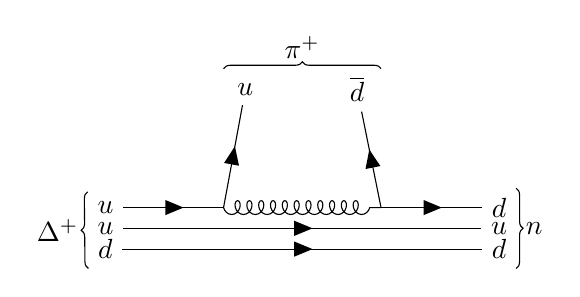
\begin{tikzpicture}
                \begin{feynman}
                    \vertex (a1) {\(u\)};
                    \vertex[right=2.5cm of a1] (a2t);
                    \vertex[left=1.cm of a2t] (a2l);
                    \vertex[right=1.cm of a2t] (a2r);
                    \vertex[right=5cm of a1] (a3) {\(d\)};

                    \vertex[below=0.75em of a1] (b1) {\(u\)};
                    \vertex[below=0.75em of a3] (b3) {\(u\)};

                    \vertex[below=0.75em of b1] (d1) {\(d\)};
                    \vertex[below=0.75em of b3] (d3) {\(d\)};

                    \vertex[above=of a2r] (c3t);
                    \vertex[left=0.25em of c3t] (c3){\( \overline d \)};
                    %\vertex[right=1em of c1t] (c1){\(\overline d\)};
                    \vertex[above=of a2l] (c1t) ;
                    \vertex[right=0.15em of c1t] (c1) {\(u\)};

                    \vertex[above=.75em of c1t] (c1tu);
                    \vertex[above=.75em of c3t] (c3tu);

                    \diagram* {
                      {[edges=fermion]
                        (a1) -- (a2l) -- (c1), (a2r) -- (a3),
                        (b1) -- (b3),
                        (d1) -- (d3),
                        (a2r) -- (c3), 
                      },

                      (a2l) -- [gluon] (a2r),
                      
                    };

                    \draw [decoration={brace}, decorate] (c1tu) -- (c3tu)
                          node [pos=0.5, above] {\(\pi^{+}\)};
                    \draw [decoration={brace}, decorate] (d1.south west) -- (a1.north west)
                          node [pos=0.5, left] {\(\Delta^{+}\)};
                    \draw [decoration={brace}, decorate] (a3.north east) -- (d3.south east) 
                          node [pos=0.5, right] {\(n\)};
                \end{feynman}
            \end{tikzpicture}
        }
    \end{center}
    \item $\Sigma^0(uds)\to\Lambda(uds)\gamma$ 
    \begin{center}
        \scalebox{1.25}{
            \begin{tikzpicture}
                \begin{feynman}
                    \vertex (a1) {\(u\)};
                    \vertex[right=2.5cm of a1] (a2t);
                    \vertex[left=1.cm of a2t] (a2l);
                    \vertex[right=1.cm of a2t] (a2r);
                    \vertex[right=5cm of a1] (a3) {\(u\)};

                    \vertex[below=0.75em of a1] (b1) {\(d\)};
                    \vertex[below=0.75em of a3] (b3) {\(d\)};

                    \vertex[below=0.75em of b1] (d1) {\(s\)};
                    \vertex[below=0.75em of b3] (d3) {\(s\)};

                    \vertex[above=of a2r] (c3t);
                    \vertex[left=0.25em of c3t] (c3){\( \gamma \)};
                    %\vertex[right=1em of c1t] (c1){\(\overline d\)};
                    \vertex[above=of a2l] (c1t) ;

                    \vertex[above=.75em of c1t] (c1tu);
                    \vertex[above=.75em of c3t] (c3tu);

                    \diagram* {
                      {[edges=fermion]
                        (a1) -- (a2) -- (a3),
                        (b1) -- (b3),
                        (d1) -- (d3),
                      },

                      (a2) -- [photon] (c3)
                      
                    };

                    \draw [decoration={brace}, decorate] (d1.south west) -- (a1.north west)
                          node [pos=0.5, left] {\(\Sigma^{0}\)};
                    \draw [decoration={brace}, decorate] (a3.north east) -- (d3.south east) 
                          node [pos=0.5, right] {\(\Lambda\)};
                \end{feynman}
            \end{tikzpicture}
        }
    \end{center} 
    \pagebreak
    \item $\pi^+(u\overbar{d})\to \mu^+ \nu_\mu$ \\[0.15in]
    \begin{center}
        \scalebox{1.25}{
            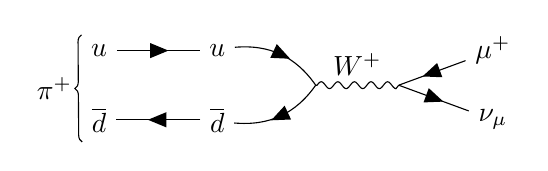
\begin{tikzpicture}
                \begin{feynman}
                   
                    \vertex (a1){\(u\)};
                    \vertex[left=1.5cm of a1] (a0u) {\(u\)};
                    \vertex[below=2.5em of a0u] (a0d) {\(\overline d\)};
                    \vertex[below=2.5em of a1] (a3) {\(\overline d\)};
                    \vertex at ($(a3)!0.5!(a1) + (1.25cm, 0)$) (a2) ;

                    \vertex[right=3em of a2] (b2);

                    \vertex[right=3.5cm of a1] (b1) {\(\mu^+\)};
                    \vertex[right=3.5cm of a3] (b3) {\(\nu_\mu\)};

                    \diagram* {

                      (a0u) -- [fermion] (a1) -- [fermion,bend left] (a2) -- [fermion, bend left] (a3) -- [fermion] (a0d),
                      (a2) -- [boson, edge label =\(W^+\)] (b2), (b1) -- [fermion] (b2) -- [fermion] (b3)

                    };
                    \draw [decoration={brace}, decorate] (a0d.south west) -- (a0u.north west)
                          node [pos=0.5, left] {\(\pi^{+}\)};
                \end{feynman}
            \end{tikzpicture}
        }
    \end{center}
\end{enumerate}
\end{solution}

\noindent\rule{7in}{1.5pt}

%%%%%%%%%%%%%%%%%%%%%%%%%%%%%%%%%%%%%%%%%%%%%%%%%%%%%%%%%%%%%%%%%%%%%%%%%%%%%%%%%%%%%%%%%%%%%%%%%%%%%%%%%%%%%%%%%%%%%%%%%%%%%%%%%%%%%%%%

\begin{problem}{1.5}
Treating the $\pi^0$ as a $uu$ bound state, draw the Feynman diagrams for:
\begin{enumerate}[label=(\alph*)]
    \item $\pi^0\to\gamma\gamma$
    \item $\pi^0\to\gamma e^+e^-$
    \item $\pi^0\to e^+e^-e^+e^-$
    \item $\pi^0\to e^+e^-$
\end{enumerate}
\end{problem}
\begin{solution}
    \begin{enumerate}[label=(\alph*)]
        \item $\pi^0\to\gamma\gamma$
        \begin{center}
            \scalebox{1.5}{
                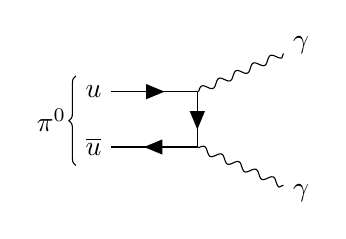
\begin{tikzpicture}
                    \begin{feynman}
                       
                        \vertex (a1) {\(u\)};
                        \vertex[right=3.75em of a1] (a2u);
                        \vertex[below=2em of a2u] (a2d);
                        \vertex[below=2em of a1] (a3) {\(\overline u\)};
    
                        \vertex[right=3.75em of a2u] (g1t);
                        \vertex[right=3.75em of a2d] (g2t);
                        \vertex[above=1em of g1t] (g1) {\(\gamma\)};
                        \vertex[below=1em of g2t] (g2) {\(\gamma\)};
    
                        \diagram* {   
                          (a1) -- [fermion] (a2u) -- [fermion] (a2d) -- [fermion] (a3),
                          (a2u) -- [photon] (g1) , (a2d) -- [photon] (g2)
                        };

                        \draw [decoration={brace}, decorate] (a3.south west) -- (a1.north west)
                              node [pos=0.5, left] {\(\pi^{0}\)};
                    \end{feynman}
                \end{tikzpicture}
            }
        \end{center}
        \item $\pi^0\to\gamma e^+e^-$
        \begin{center}
            \scalebox{1.5}{
                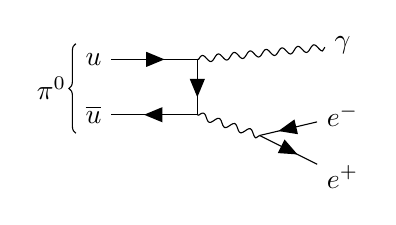
\begin{tikzpicture}
                    \begin{feynman}
                       
                        \vertex (a1) {\(u\)};
                        \vertex[right=3.75em of a1] (a2u);
                        \vertex[below=2em of a2u] (a2d);
                        \vertex[below=2em of a1] (a3) {\(\overline u\)};
    
                        %\vertex[right=2.25em of a2u] (g1u);
                        \vertex at ($ (a2u) + (5.25em,0.5em) $) (g1u_t) {\(\gamma\)};
                        \vertex at ($ (a2u) + (2.25em,0.75em) $) (g1u);
                        \vertex at ($ (a2d) + (2.25em,-0.75em) $) (g2d);
                        %\vertex[right=2.25em of a2d] (g2d);

                        \vertex at ($ (g1u) + (3em,1.5em) $) (e1);
                        \vertex at ($ (g2d) + (3em,-1.5em) $) (e4) {\(e^+\)};
                        \vertex at ($ (e1)!.33!(e4) $) (e2);
                        \vertex at ($ (e1)!.66!(e4) $) (e3) {\(e^-\)};
    
                        \diagram* {   
                          (a1) -- [fermion] (a2u) -- [fermion] (a2d) -- [fermion] (a3),
                          (a2u) -- [photon] (g1u_t) , (a2d) -- [photon] (g2d) ,
                          (e3) -- [fermion] (g2d) -- [fermion]  (e4)
                        };

                        \draw [decoration={brace}, decorate] (a3.south west) -- (a1.north west)
                              node [pos=0.5, left] {\(\pi^{0}\)};
                    \end{feynman}
                \end{tikzpicture}
            }
        \end{center}
        \item $\pi^0\to e^+e^-e^+e^-$
        \begin{center}
            \scalebox{1.5}{
                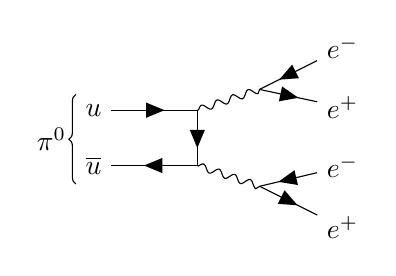
\begin{tikzpicture}
                    \begin{feynman}
                       
                        \vertex (a1) {\(u\)};
                        \vertex[right=3.75em of a1] (a2u);
                        \vertex[below=2em of a2u] (a2d);
                        \vertex[below=2em of a1] (a3) {\(\overline u\)};
    
                        %\vertex[right=2.25em of a2u] (g1u);
                        \vertex at ($ (a2u) + (2.25em,0.75em) $) (g1u);
                        \vertex at ($ (a2d) + (2.25em,-0.75em) $) (g2d);
                        %\vertex[right=2.25em of a2d] (g2d);

                        \vertex at ($ (g1u) + (3em,1.5em) $) (e1) {\(e^-\)};
                        \vertex at ($ (g2d) + (3em,-1.5em) $) (e4) {\(e^+\)};
                        \vertex at ($ (e1)!.33!(e4) $) (e2) {\(e^+\)};
                        \vertex at ($ (e1)!.66!(e4) $) (e3) {\(e^-\)};
    
                        \diagram* {   
                          (a1) -- [fermion] (a2u) -- [fermion] (a2d) -- [fermion] (a3),
                          (a2u) -- [photon] (g1u) , (a2d) -- [photon] (g2d) ,
                          (e1) -- [fermion] (g1u) -- [fermion]  (e2) , (e3) -- [fermion] (g2d) -- [fermion]  (e4)
                        };

                        \draw [decoration={brace}, decorate] (a3.south west) -- (a1.north west)
                              node [pos=0.5, left] {\(\pi^{0}\)};
                    \end{feynman}
                \end{tikzpicture}
            }
        \end{center}
        \item $\pi^0\to e^+e^-$
        \begin{center}
            \scalebox{1.25}{
                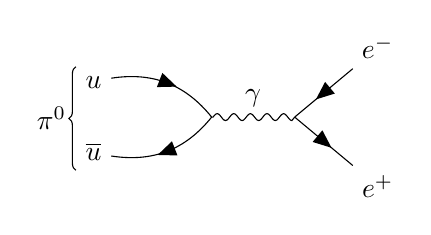
\begin{tikzpicture}
                    \begin{feynman}
                       
                        \vertex (a1){\(u\)};
                        \vertex[below=2.5em of a1] (a3) {\(\overline u\)};
                        \vertex at ($(a3)!0.5!(a1) + (1.5cm, 0)$) (a2) ;
    
                        \vertex[right=3em of a2] (b2);
    
                        \vertex at ($(a2) + (6em,2.5em)$) (b1) {\(e^-\)};
                        \vertex at ($(a2) + (6em,-2.5em)$) (b3) {\(e^+\)};
                        %\vertex[right=4.5cm of a1] (b1) {\(\mu^+\)};
                        %\vertex[right=4.5cm of a3] (b3) {\(\nu_\mu\)};
    
                        \diagram* {
    
                          (a1) -- [fermion,bend left] (a2) -- [fermion, bend left] (a3) ,
                          (a2) -- [boson, edge label =\(\gamma\)] (b2), (b1) -- [fermion] (b2) -- [fermion] (b3)
    
                        };
                        \draw [decoration={brace}, decorate] (a3.south west) -- (a1.north west)
                              node [pos=0.5, left] {\(\pi^{0}\)};
                    \end{feynman}
                \end{tikzpicture}
            }
        \end{center}
    \end{enumerate}
\end{solution}

\noindent\rule{7in}{1.5pt}

%%%%%%%%%%%%%%%%%%%%%%%%%%%%%%%%%%%%%%%%%%%%%%%%%%%%%%%%%%%%%%%%%%%%%%%%%%%%%%%%%%%%%%%%%%%%%%%%%%%%%%%%%%%%%%%%%%%%%%%%%%%%%%%%%%%%%%%%

\begin{problem}{1.6}
Particle interactions fall into two main categories, scattering processes and annihilation processes, as indicated by the Feynman diagrams below.
\begin{center}
    \scalebox{1.5}{
    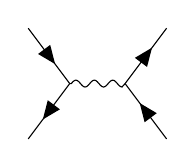
\begin{tikzpicture}
        \begin{feynman}
            \vertex (a1);
            \vertex[below=4em of a1] (a3);
            \vertex[right=1.5em of a3] (a2t);
            \vertex[above=2em of a2t] (a2);
    
            \vertex[right=2em of a2] (b2);
            \vertex[right=5em of a1] (b1);
            \vertex[right=5em of a3] (b3);
    
            \diagram* {
                {[edges=fermion]
                  (a1) -- (a2) -- (a3),
                  (b3) -- (b2) -- (b1)
                },
                (a2) -- [boson] (b2)
            };
        \end{feynman}
    \end{tikzpicture} \hspace{0.15in}
    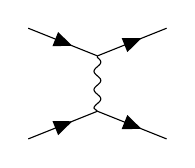
\begin{tikzpicture}
        \begin{feynman}
            \vertex (a1);
            \vertex[right=5em of a1] (a3);
            \vertex[right=2.5em of a1] (a2t);
            \vertex[below=1em of a2t] (a2);
    
            \vertex[below=4em of a1] (b1);
            \vertex[right=5em of b1] (b3);
            \vertex[right=2.5em of b1] (b2t);
            \vertex[above=1em of b2t] (b2);

            \diagram* {
                {[edges=fermion]
                  (a1) -- (a2) -- (a3),
                  (b1) -- (b2) -- (b3)
                },
                (a2) -- [boson] (b2)
            };
            
        \end{feynman}
    \end{tikzpicture}
    }
\end{center}
Draw the lowest-order Feynman diagrams for the scattering and/or annihilation processes:
\begin{enumerate}[label=(\alph*)]
    \item $e^-e^- \to e^-e^-$
    \item $e^+e^- \to \mu^+\mu^-$
    \item $e^+e^- \to e^+e^-$
    \item $e^-\nu_e \to e^-\nu_e$
    \item $e^-\overbar{\nu_e} \to e^-\overbar{\nu_e}$
\end{enumerate}
\end{problem}
\begin{solution}
\begin{enumerate}[label=(\alph*)]
    \item $e^-e^- \to e^-e^-$
    \begin{center}
        \scalebox{1.5}{
            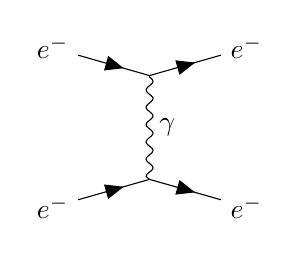
\begin{tikzpicture}
                \begin{feynman}
                    \vertex (a2) ;
                    \vertex at ($(a2) + (-3.5em,1em) $) (a1) {$e^-$};
                    \vertex at ($(a2) + (3.5em,1em) $) (a3) {$e^-$};
            
                    \vertex[below=3.75em of a2] (b2);        
                    \vertex at ($(b2) + (-3.5em,-1em) $) (b1) {$e^-$};
                    \vertex at ($(b2) + (3.5em,-1em) $) (b3) {$e^-$};
            
                    \diagram* {
                        {[edges=fermion]
                          (a1) -- (a2) -- (a3),
                          (b1) -- (b2) -- (b3)
                        },
                        (a2) -- [boson, edge label =\(\gamma\)] (b2)
                    };
                    
                \end{feynman}
            \end{tikzpicture}
        }
    \end{center}
    \item $e^+e^- \to \mu^+\mu^-$
    \begin{center}
        \scalebox{1.25}{
            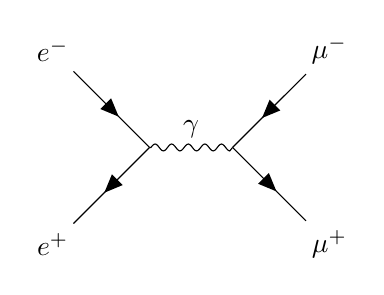
\begin{tikzpicture}
                \begin{feynman}
                    
                    \vertex (g1);
                    \vertex at ($(g1) + (-3.5em,3.5em) $) (e1) {\(e^-\)};
                    \vertex at ($(g1) + (-3.5em,-3.5em) $) (e2) {\(e^+\)};

                    \vertex at ($(g1) + (3em,0)$) (g2) ;
                    \vertex at ($(g2) + (3.5em,3.5em) $) (m1) {\(\mu^-\)};
                    \vertex at ($(g2) + (3.5em,-3.5em) $) (m2) {\(\mu^+\)};
                    \diagram* {
                        {[edges=fermion]
                          (e1) -- (g1) -- (e2),
                          (m1) -- (g2) -- (m2)
                        },
                        (g1) -- [boson, edge label =\(\gamma\)] (g2)
                    };

                \end{feynman}
            \end{tikzpicture}
        }
    \end{center}
    \item $e^+e^- \to e^+e^-$
    \item $e^-\nu_e \to e^-\nu_e$
    \item $e^-\overbar{\nu_e} \to e^-\overbar{\nu_e}$
\end{enumerate}
\end{solution}

\noindent\rule{7in}{1.5pt}

%%%%%%%%%%%%%%%%%%%%%%%%%%%%%%%%%%%%%%%%%%%%%%%%%%%%%%%%%%%%%%%%%%%%%%%%%%%%%%%%%%%%%%%%%%%%%%%%%%%%%%%%%%%%%%%%%%%%%%%%%%%%%%%%%%%%%%%%

\begin{problem}{1.7}
High-energy muons traversing matter lose energy according to
\begin{align*}
    -\frac{1}{\rho} \frac{\dif E}{\dif x} \approx a + bE 
\end{align*}
where $a$ is due to ionisation energy loss and $b$ is due to the bremsstrahlung and $e^+e^-$ pair-production processes. 
For standard rock, taken to have $A = 22, Z = 11$ and $\rho = 2.65 \unit{\gram\centi\metre^{-3}}$ , the parameters $a$ and $b$ depend only weakly on 
the muon energy and have values $a \approx 2.5 \MeV\unit{\gram^{-1}\centi\metre^2}$ and $b \approx \num{3.5e-6} \unit{\gram^{-1}\centi\metre^2}$.
\begin{enumerate}[label=(\alph*)]
    \item At what muon energy are the ionisation and bremsstrahlung/pair production processes equally important?
    \item Approximately how far does a 100 GeV cosmic-ray muon propagate in rock?
\end{enumerate}
\end{problem}
\begin{solution}
%Using the given approximation of $\dif E / \dif x$, one could solve the differential equation of $E(x)$ as
%\begin{align*}
%    -\frac{1}{\rho} \frac{\dif E}{\dif x} \approx a + bE  &\implies - \frac{\dif E}{\rho \left( a+bE \right)} \approx \dif x  \\[0.15in]
%                                                          &\implies  E(x) \approx \frac{c}{\rho b} e^{\rho b x} - \frac{a}{b}
%\end{align*}
\begin{enumerate}[label=(\alph*)]
    \item One could assume that ionisation and bremsstrahlung/pair production processes become equally important for a certain energy scale $E^\ast$ when $a \simeq bE^\ast$.
    Such $E^\ast \simeq a/b$ can be calculated as $\sim 700 \GeV$.
    \item Using the values given, 

    \begin{align*}
        - \frac{\dif E}{\dif x} &\approx a \rho + b \rho  E \impliedby \left( a\rho \sim \num{6.6}\MeV/\text{cm} \text{ , } b \rho \sim \num{9.275e-6}/\text{cm} \right) \\[0.15in]
                                &\simeq 7.52 \MeV/\text{cm} 
    \end{align*}\\
    which shows that a 100 GeV muon will go through around 132 metres of rock.
\end{enumerate}
\end{solution}

\noindent\rule{7in}{1.5pt}

%%%%%%%%%%%%%%%%%%%%%%%%%%%%%%%%%%%%%%%%%%%%%%%%%%%%%%%%%%%%%%%%%%%%%%%%%%%%%%%%%%%%%%%%%%%%%%%%%%%%%%%%%%%%%%%%%%%%%%%%%%%%%%%%%%%%%%%%

\begin{problem}{1.8}
Tugsten has a radiation length of $X_0=0.35$ cm and a critical energy of $E_c = 7.97$ MeV. Roughly what thickness of tungsten is required to fully contain a 500 GeV electromagnetic shower from an electron?
\end{problem}
\begin{solution}
Getting $x_\text{max}$ for the given situation, one obtains :

\begin{align*}
    x_{\text{max}} = \frac{1}{\ln 2}\ln\left( \frac{E}{E_c}\right) = \frac{1}{\ln 2}\ln\left( \frac{500 \GeV}{7.97 \MeV}\right) \sim 16
\end{align*}\\
Thus, roughly around $x_\text{max}X_0 \simeq 5.6 \unit{\centi\metre}$ of tungsten would be able to contain a 500 GeV electromagnetic shower from an electron.\\
\end{solution} 
\noindent\rule{7in}{1.5pt}

%%%%%%%%%%%%%%%%%%%%%%%%%%%%%%%%%%%%%%%%%%%%%%%%%%%%%%%%%%%%%%%%%%%%%%%%%%%%%%%%%%%%%%%%%%%%%%%%%%%%%%%%%%%%%%%%%%%%%%%%%%%%%%%%%%%%%%%%

\begin{problem}{1.9}
The CPLEAR detector consisted of: tracking detectors in a magnetic field of 0.44 T; and electromagnetic calorimeter;
and Čerenkov detectors with a radiator of refractive index $n=1.25$ used to distinguish $\pi^\pm$ from $K^\pm$.

A charged particle travelling perpendicular to the direction of the magnetic field leaves a track with a
measured radius of curvature of $R=4$m. If it is observed to give a Čerenkov signal, is it 
possible to distinguish between the particle being a pion or kaon? Take $m_\pi \approx 140 \MeV /\text{c}^2$ and $m_K \approx 494 \MeV /\text{c}^2$ 
\end{problem}
\begin{solution}
First, the momentum could be extracted from the fact that the charged particles are travelling perpendicular ($\lambda =0 $) to the 0.44 T magnetic field, 
which eventually gives $p=0.3BR=0.528\GeV$. The threshold mass for Čerenkov radiation in this case would be,

\begin{align*}
    \sqrt{n^2-1} p = 0.75 \times p = 0.396 \GeV
\end{align*}\\
thus in such situation it would be able to identity whether the track corresponds to a pion or kaon, as only $m_\pi$ is smaller than the threshold Čerenkov radiation mass.
\end{solution}

\noindent\rule{7in}{1.5pt}

%%%%%%%%%%%%%%%%%%%%%%%%%%%%%%%%%%%%%%%%%%%%%%%%%%%%%%%%%%%%%%%%%%%%%%%%%%%%%%%%%%%%%%%%%%%%%%%%%%%%%%%%%%%%%%%%%%%%%%%%%%%%%%%%%%%%%%%%

\begin{problem}{1.10}
In a fixed-target pp experiment, what proton energy would be required to achieve the same centre-of-mass energy as the LHC, which will ultimately operate at 14 TeV.
\end{problem}
\begin{solution}
Let the four-momentum of the beam proton and the fixed target proton as $p_1 = (E,0,0,p)$ and $p_2 = (m_p,0,0,0)$. Using the following expression of the centre-of-mass energy $\sqrt{s}$, the proton energy $E$ to satisfy the required situation would be :

\begin{align*}
    \sqrt{s} = (p_1 + p_2) ^2 &= 2m_p^2 + 2 p_1 \cdot p_2 \\[0.15in]
                              &= 2m_p \left( m_p + E \right) = 14 \text{ TeV} \implies \boxed{E \simeq 7.4 \text{ PeV}}
\end{align*}
\end{solution} 

\noindent\rule{7in}{1.5pt}
    
%%%%%%%%%%%%%%%%%%%%%%%%%%%%%%%%%%%%%%%%%%%%%%%%%%%%%%%%%%%%%%%%%%%%%%%%%%%%%%%%%%%%%%%%%%%%%%%%%%%%%%%%%%%%%%%%%%%%%%%%%%%%%%%%%%%%%%%%

\begin{problem}{1.11}
At the LEP $e^+e^-$ collider, which had a circumference of 27 km, the electron and positron beam currents were both 1.0 mA. Each beam consisted of four equally spaced bunches of electrons/positrons. The bunches had an effective area of $\num{1.8e4}\unit{\micro\metre^2}$.
Calculate the instantaneous luminosity on the assumption that the beams collided head-on.
\end{problem}
\begin{solution}
The instantaneous luminosity $\mathcal{L}$ could be computed as,

\begin{align*}
    \mathcal{L} = f\frac{n_1n_2}{4\pi \sigma_x \sigma_y}
\end{align*}\\
As the problem states, the given effective area $\num{1.8e4} \unit{\micro\meter^2}=\num{1.8e-4} \unit{\centi\meter^2}$ of the bunches will correspond to $\sigma_x \sigma_y$. In this case, the bunches are seperated $27/4 = 6.75 \unit{km}$ and as the leptons were accelerated $\sim 0.99c$, the temporal separation between the beams will be $\simeq 5 \unit{\micro\second}$ where relativistic effects are folded in, thus the collision frequency will be $f \simeq 200 \unit{\kilo\hertz}$. Using the beam current $\num{1.0e-3}\unit{C\cdot s^{-1}}$, the number of electrons can be derived using

\begin{align*}
    n_1 = n_2 = \frac{\num{1.0}\unit{\milli\ampere}}{ef}=\frac{\num{1.0e-3}\unit{C\cdot s^{-1}}}{\num{1.62e-19}\unit{C}} \times 5 \unit{\micro\second} \simeq \num{3.5e10}
\end{align*}\\
Then using all the numbers derived, the instantaneous luminosity can be calculated as,

\begin{align*}
    \mathcal{L} = \num{2.0e5} \unit{s^{-1}} \times \frac{\left( \num{3.5e10}\right)^2}{\num{1.8e-4}\unit{\centi\meter^2}} \simeq \num{1.3e30} \unit{cm^{-2}\cdot s^{-1}}
\end{align*}
\end{solution}\\
\noindent\rule{7in}{2.8pt}
\section{Underlying Concepts}
\begin{problem}{2.1}
When expressed in natural units the lifetime of the W boson is approximately $\tau \approx 0.5\GeV^{-1}$. What is the corresponding value in S.I. units?
\end{problem}
\begin{solution}
In natural units, $\hbar = \num{1.055e-34}\unit{J\cdot s} = \num{6.582e-25} \unit{GeV\cdot s}$ which is, $1 \GeV^{-1} = \num{6.582e-25} \unit{s}$.
Thus the lifetime of the W boson in S.I. units can be written as, $\boxed{\tau \simeq \num{3.291e-25} \unit{s}}$.\\
\end{solution} 
\noindent\rule{7in}{1.5pt}

%%%%%%%%%%%%%%%%%%%%%%%%%%%%%%%%%%%%%%%%%%%%%%%%%%%%%%%%%%%%%%%%%%%%%%%%%
% Problem 2
%%%%%%%%%%%%%%%%%%%%%%%%%%%%%%%%%%%%%%%%%%%%%%%%%%%%%%%%%%%%%%%%%%%%%%%%%%%%%%%%%%%%%%%%%%%%%%%%%%%%%%%%%%%%%%%%%%%%%%%%%%%%%%%%%%%%%%%%

\begin{problem}{2.2}
A cross section is measured to be 1 pb; convert this to natural units.
\end{problem}
\begin{solution}
Taking note that $\hbar c = 0.197 \GeV \text{ fm}$, which is $0.197 \GeV = 1 \unit{\femto\metre}^{-1}$

\begin{align*}
    1 \pb = 10^{-10} \text{ fm}^2 = 10^{-10} \times \left( \frac{1}{0.197} \right)^2 \GeV^{-2} = \boxed{\num{2.57e-9}\GeV^{-2}}
\end{align*}
\end{solution} 
\noindent\rule{7in}{1.5pt}

%%%%%%%%%%%%%%%%%%%%%%%%%%%%%%%%%%%%%%%%%%%%%%%%%%%%%%%%%%%%%%%%%%%%%%%%%

\begin{problem}{2.3}
Show that the process $\gamma\to e^+ e^-$ can not occur in vacuum.
\end{problem}
\begin{solution}
If it were so, such process should occur in any frame. Let such frame as the rest frame of
\end{solution} 
\noindent\rule{7in}{1.5pt}

%%%%%%%%%%%%%%%%%%%%%%%%%%%%%%%%%%%%%%%%%%%%%%%%%%%%%%%%%%%%%%%%%%%%%%%%%

\begin{problem}{2.4}
A particle of mass 3 GeV is travelling in the positive z-direction with momentum 4 GeV. What are its energy and velocity?
\end{problem}
\begin{solution}
Using the relation of $m^2=E^2- | \boldp |^2 $, one gets $E^2 = 25 \GeV^2$ thus the energy is $\boxed{E=5\GeV}$. Now considering the relation of $|\boldp|=E\beta$, it is seen that $\beta = |\boldp|E^{-1}=0.8$ thus the velocity is $\boxed{0.8c}$.\\ 
\end{solution} 
\noindent\rule{7in}{1.5pt}

%%%%%%%%%%%%%%%%%%%%%%%%%%%%%%%%%%%%%%%%%%%%%%%%%%%%%%%%%%%%%%%%%%%%%%%%%

\begin{problem}{2.5}
In the laboratory frame, denoted $\Sigma$, a particle travelling in the z-direction has momentum $\mathbf{p}=p_z \hat{\mathbf
z}$ and energy $E$.
\begin{enumerate}[label=(\alph*)]
    \item Use the Lorentz transformation to find expressions for the momentum $p'_z$ and energy $E'$ of the particle in a frame $\Sigma'$ which is moving in a velopcity $\mathbf{v}=+v\hat{\mathbf
    z}$ relative to $\Sigma$, and show that $E^2-p_z^2=(E')^2-(p'_z)^2$.
    \item For a system of particles, prove that the total four-momentum squared, 
    \begin{align*}
        p^\mu p_\mu \equiv  \left( \sum_{i}E_i \right)^2 - \left( \sum_{i}\mathbf{p}_i \right)^2
    \end{align*}
    is invariant under Lorentz transformations.
\end{enumerate}
\end{problem}

\begin{solution}
    \begin{enumerate}[label=(\alph*)]   
        \item Let the four-momentum of the given particle in the frame $\Sigma$ and $\Sigma'$ as $p=(E,0,0,p_z),p'=(E',\boldp')$ respectively. Denoting the corresponding matrix representation of the given Lorentz transformation as $\boldsymbol{\Lambda}$, one could write down the transformation of $p$ as,
        
        \begin{align*}
            p' = \boldsymbol{\Lambda} p \implies p'^\mu &= \Lambda^{\mu}_\nu p^\nu \\[0.1in]
                   &= \begin{pmatrix}
                    \gamma       & 0 & 0 & -\gamma\beta \\
                    0            & 1 & 0 & 0            \\
                    0            & 0 & 1 & 0            \\
                    -\gamma\beta & 0 & 0 & \gamma      
                   \end{pmatrix}
                   \begin{pmatrix}
                    E \\
                    0 \\
                    0 \\
                    p_z 
                   \end{pmatrix} = \gamma
                   \begin{pmatrix}
                    E-\beta p_z \\ 0 \\ 0 \\ -E\beta +  p_z \\
                   \end{pmatrix} 
        \end{align*}\\
        which implies that $E' = \gamma \left( E-\beta p_z \right)$ and $p_z'=-\gamma(E\beta-p_z)$. Using such expression of $p'$, one could show that : 

        \begin{align*}
            \left(E'\right)^2 - \left(p_z'\right)^2 &= \gamma^2 (E-\beta p_z)^2 - \gamma^2 (E\beta - p_z)^2 \\[0.1in]
                                                    &= \gamma^2 \left[  \left( E-\beta p_z \right)^2 - \left(E\beta - p_z \right)^2 \right] \\[0.1in]
                                                    &= \gamma^2 \left[  \left( E-\beta p_z + E\beta - p_z \right) \left( E-\beta p_z - E\beta + p_z  \right) \right] \\[0.1in]
                                                    &= \gamma^2 (1+\beta)(1-\beta) (E-p_z)(E+p_z) = E^2 - p_z^2 \qed
        \end{align*}
        \item 
    \end{enumerate}
\end{solution} 
\noindent\rule{7in}{1.5pt}

%%%%%%%%%%%%%%%%%%%%%%%%%%%%%%%%%%%%%%%%%%%%%%%%%%%%%%%%%%%%%%%%%%%%%%%%%

\begin{problem}{2.6}\label{p2.6}
   For the decay $a\to1+2$, show that the mass of the particle $a$ can be expressed as 
   \begin{align*}
        m_a^2 = m_1^2+m_2^2 + 2E_1E_2\left( 1 - \beta_1\beta_2 \cos\theta \right)
   \end{align*}
   where $\beta_1$ and $\beta_2$ are the velocities of the daughter particles and $\theta$ is the angle between them.
\end{problem}
    
\begin{solution}
    Let the four-momenta of the daughters as $p_i = \left( E_i,\boldp_i \right)$ for $i=1,2$. Momentum conservation states that $p_a = p_1 + p_2$ where $p_a$ is the four-momentum of the mother particle.
    Squaring both sides, one obtains 
    \begin{align*}
        p_a \cdot p_a = m_a^2 &= \left( p_1 + p_2 \right)^2 \\[0.1in]
                              &= p_1 \cdot p_1 + p_2 \cdot p_2 + 2 p_1 \cdot p_2 \\[0.1in]
                              &= m_1^2 + m_2^2 + 2 (E_1E_2 - \boldp_1 \cdot \boldp_2) \\[0.1in]
                              &= m_1^2 + m_2^2 + 2 (E_1E_2 - |\boldp_1||\boldp_2|\cos\theta  ) \\[0.1in]
                              &= m_1^2 + m_2^2 + 2 (E_1E_2 - E_1\beta_1E_2\beta_2\cos\theta  ) \\[0.1in]
                              &= m_1^2+m_2^2 + 2E_1E_2\left( 1 - \beta_1\beta_2 \cos\theta \right) \qed 
    \end{align*}
\end{solution} 
    
\noindent\rule{7in}{1.5pt}

%%%%%%%%%%%%%%%%%%%%%%%%%%%%%%%%%%%%%%%%%%%%%%%%%%%%%%%%%%%%%%%%%%%%%%%%%

\begin{problem}{2.7}
In a collider experiment, $\Lambda$ baryons can be identified from the decay $\Lambda\to\pi^-p$, which gives rise to a displaced vertex in a tracking detector. In a particular decay, the momenta of the $\pi^+$ and $p$ are measured to be $0.75 \GeV$ and $4.25 \GeV$ respectively, and the opening angle between the tracks is $9^\circ$. The masses of the pion and proton are $189.6 \MeV$ and $938.3 \MeV$.
\begin{enumerate}[label=(\alph*)]
    \item Calculate the mass of the $\Lambda$ baryon.
    \item On average, $\Lambda$ baryons of this energy are observed to decay at a distance of 0.35 m from the point of production. Calculate the lifetime of the $\Lambda$.
\end{enumerate}
\end{problem}
\begin{solution}
\begin{enumerate}[label=(\alph*)]
    \item Let the four-momenta of $\pi^-,p$ as $p_\pi = (\num{0.75}\GeV,\boldp_\pi)$,$p_p = (\num{4.25}\GeV,\boldp_p)$ respectively, which gives $p_\Lambda = p_\pi + p_p = (5 \GeV,\boldp_\pi + \boldp_p)$ as the four-momenta of $\Lambda$. 
    Using the mass of the pion and proton, one could obtain 

    \begin{align*}
        \left| \boldp_\pi \right|^2  &= (0.75 \GeV)^2 - m_\pi^2 \simeq 0.5265 \GeV^2 \implies  \left| \boldp_\pi \right| \simeq  0.725 \GeV \\
        \left| \boldp_p \right|^2    &= (4.25 \GeV)^2 - m_p^2 \simeq 17.18 \GeV^2 \implies  \left| \boldp_\pi \right| \simeq 4.144 \GeV
    \end{align*}\\
    The mass of the $\Lambda$ baryon $m_\Lambda$ can be acquired as : 

    \begin{align*}
        m_\Lambda^2 = p_\Lambda \cdot p_\Lambda &= (5 \GeV)^2 - \left| \boldp_\pi + \boldp_p \right|^2 \\[0.15in]
                                              &= (5 \GeV)^2 - \left[ \left| \boldp_\pi \right|^2 +  \left| \boldp_p \right|^2 + 2  \left| \boldp_\pi \right| \left| \boldp_p \right| \cos 9^\circ  \right] \\[0.15in]
                                              &= (5 \GeV)^2 - \left[  0.5265+  17.18  + 2 \cdot 0.725 \cdot 4.144 \cdot  0.98  \right] \GeV^2 \\[0.15in] 
                                              &\simeq 1.35 \GeV^2 \implies \boxed{m_\Lambda \simeq 1.16 \GeV}
    \end{align*}\\
    which agrees well with experimental values.
    \item Let the lifetime and $\beta$ of $\Lambda$ as $\tau_\Lambda$ and $\beta_\Lambda$ then one could realize that $c\beta_\Lambda \tau_\Lambda \sim 0.35 \unit{\metre}$.
    $\beta_\Lambda$ can be simply derived using $\beta_\Lambda = \left| \boldp_\Lambda \right|/E_\Lambda \simeq 0.97$. Thus the lifetime of $\Lambda$ becomes $\boxed{\tau_\Lambda \simeq \num{0.12e-8} \unit{s}}$
\end{enumerate}
\end{solution} 
\noindent\rule{7in}{1.5pt}


%%%%%%%%%%%%%%%%%%%%%%%%%%%%%%%%%%%%%%%%%%%%%%%%%%%%%%%%%%%%%%%%%%%%%%%%%

\begin{problem}{2.8}
    In the laboratory frame, a proton with total energy E collides with proton at rest. Find the minimum proton energy such that process
    \begin{align*}
        p+p \to p+p+\bar{p}+\bar{p}
    \end{align*}
    is kinematically allowed.
\end{problem}
\begin{solution}
        
\end{solution} 

\noindent\rule{7in}{1.5pt}

%%%%%%%%%%%%%%%%%%%%%%%%%%%%%%%%%%%%%%%%%%%%%%%%%%%%%%%%%%%%%%%%%%%%%%%%%

\begin{problem}{2.9}
Find the maximum opening angle between the photons produced in the decay $\pi^0\to\gamma\gamma$ if the energy of the neutral pion is 10 GeV, given that $m_{\pi^0}=135$ MeV.
\end{problem}
\begin{solution}
Using the results derived in Problem~\ref{p2.6} and taking account on the fact that photons are massless, one could write down 

\begin{align*}
    m_{\pi_0^2} = 2E_1E_2 \left( 1- \beta_1 \beta_2 \cos \theta \right) = 2E_1E_2 \left( 1- \cos\theta \right) \implies \cos \theta =  \frac{m_{\pi_0}^2}{2E_1E_2} - 1  
\end{align*}\\
Taking account that $E_1+E_2 = 10 \GeV$, let $E_1=E$ and express $\theta$ in terms of $E$ as,

\begin{align*}
    \cos \theta =  \frac{m_{\pi_0}^2}{2E(10-E)} - 1  
\end{align*}\\
In the range of $E\in[0,10]\GeV$ the RHS of the above identity will take a local minimum when $E=5\GeV$ which will give the maximum value of $\theta$, which will be denoted as $\theta^\ast$. One could get $\theta^\ast$ as,

\begin{align*}
    \cos \theta^\ast = \frac{\left( \num{1.35e-1}\GeV \right)^2}{100 \GeV^2} - 1 = -0.99981775 \implies \boxed{\theta^\ast \simeq  178.906099^\circ}
\end{align*}\\
which is nearly back-to-back.
\end{solution} 

\noindent\rule{7in}{1.5pt}

%%%%%%%%%%%%%%%%%%%%%%%%%%%%%%%%%%%%%%%%%%%%%%%%%%%%%%%%%%%%%%%%%%%%%%%%%

\begin{problem}{2.10}
The maximum of the $\pi^-p$ cross section, which occurs at $p_\pi=300$ MeV, corresponds to the resonant production of the $\Delta^0$ baryon (i.e. $\sqrt{s}=m_\Delta$). What is the mass of the $\Delta$?
\end{problem}
\begin{solution}
        
\end{solution} 

\noindent\rule{7in}{1.5pt}

%%%%%%%%%%%%%%%%%%%%%%%%%%%%%%%%%%%%%%%%%%%%%%%%%%%%%%%%%%%%%%%%%%%%%%%%%

\begin{problem}{2.11}
   Tau-leptons are produced in the process $e^+e^-\to\tau^+\tau^-$ at a centre-of-mass energy of 91.2 GeV. The angular distribution of the $\pi^-$ from the decay $\tau^-\to\pi^-\nu_\tau$ is 
   \begin{align*}
        \frac{\dif N}{ \dif \left(\cos\theta^\ast\right)} \varpropto 1 + \cos\theta^\ast
   \end{align*} 
   where $\theta^\ast$ is the polar angle of the $\pi^-$ in the tau-lepton rest frame, relative to the direction defined by the $\tau$ spin. Determine the laboratory frame energy distribution of the $\pi^-$ for the cases where the tau lepton spin is (i) \textit{aligned with} or (ii) \textit{opposite} to its direction of flight.
\end{problem}
\begin{solution}
            
\end{solution} 
    
\noindent\rule{7in}{1.5pt}

%%%%%%%%%%%%%%%%%%%%%%%%%%%%%%%%%%%%%%%%%%%%%%%%%%%%%%%%%%%%%%%%%%%%%%%%%


\begin{problem}{2.12}
   For the process $1+2 \to 3+4$, the Mandelstam variables $s,t$ and $u$ are defined as $s=(p_1+p_2)^2,t=(p_1-p_3)^2$ and $u=(p_1-p_4)^2$. Show that
   \begin{align*}
        s+t+u = m_1^2+m_2^2+m_3^2+m_4^2.
   \end{align*} 
\end{problem}
\begin{solution}
    By definition of the Mandelstam variables, one could express $(s+t+u)$ as 
    
    \begin{align*}
        s+t+u &= (p_1+p_2)^2 + (p_1-p_3)^2 + (p_1-p_4)^2\\[0.1in]
              &= \sum_i p_i \cdot p_i  + 2p_1\cdot p_1  + 2p_1\cdot p_2 -2 p_1 \cdot p_3 - 2 p_1 \cdot p_4  \\  
              &= \sum_i m_i^2 + 2p_1\cdot(p_1+p_2-p_3-p_4) \\
              &= \sum_i m_i^2 \qed
    \end{align*}\\
    The fact that in any frame $p^\mu p_\mu =m^2$ for a particle with mass $m$ is used in the third identity, and in the last step the conservation of momentum $p_1+p_2 = p_3+p_4$ is used. 
\end{solution} 
    
\noindent\rule{7in}{1.5pt}

%%%%%%%%%%%%%%%%%%%%%%%%%%%%%%%%%%%%%%%%%%%%%%%%%%%%%%%%%%%%%%%%%%%%%%%%%

\begin{problem}{2.13}
 At the HERA collider, 27.5 GeV electrons were collided head-on with 820 GeV protons. Calculate the centre-of-mass energy.
\end{problem}
\begin{solution}
    Let the four-momentum of the electron and proton as $p_e = (E_e,\mathbf{p}_e),$ $p_p = (E_p,\mathbf{p}_p)$ respectively. The centre-of-mass energy $\sqrt{s}$ can be expressed as,
    
    \begin{align*}
        s &= \left( p_e + p_p \right)^2 = p_e\cdot p_e + p_p \cdot p_p + 2 p_e \cdot p_p \\[0.1in]
          &= m_e^2 + m_p^2 + 2 \left( E_e E_p - \boldp_e \cdot \boldp_p \right) \\[0.1in]
          &= m_e^2 + m_p^2 + 2 \left( E_eE_p + \left| \boldp_e \right| \left| \boldp_p \right| \right) \simeq 4 E_e E_p \quad \quad \left(  |\boldp_i|^2 = E_i^2 - m_i^2 \sim E_i^2  \right)
    \end{align*}\\
    As the collision is occuring head-on, one could say that $\boldp_e \cdot \boldp_p =- \left| \boldp_e \right| \left| \boldp_p \right| $ which was used in the last identity.
    Looking upon the order of the variables, $m_e \simeq 0.5 \MeV, m_p \simeq 93.8 \MeV$ and $E_e = 27.5 \GeV, E_p = 820 \GeV$ for an approximation it is okay to consider $m_e,m_p\sim 0$. Thus the centre-of-mass energy $\boxed{\sqrt{s}\simeq 300 \GeV}$ when all the needed values are plugged in.
\end{solution}
    
\noindent\rule{7in}{1.5pt}

%%%%%%%%%%%%%%%%%%%%%%%%%%%%%%%%%%%%%%%%%%%%%%%%%%%%%%%%%%%%%%%%%%%%%%%%%

\begin{problem}{2.14}
Consider the Compton scattering of a photon of momentum $\mathbf{k}$ and energy $E = \left| \mathbf{k} \right| = \mathbf{k}$ from an electron at rest.
Writing the four-momenta of the scattered photon and electron respectively as $k'$ and $p'$, conservation of four- momentum is expressed as $k + p = k' + p'$.
Use the relation $p'^2 = m_e^2$ to show that the energy of the scattered photon is given by
\begin{align*}
    E' = \frac{E}{1+\left( E/m_e \right)\left( 1-\cos\theta \right)}
\end{align*}
\end{problem}
\begin{solution}
            
\end{solution}
    
\noindent\rule{7in}{1.5pt}

%%%%%%%%%%%%%%%%%%%%%%%%%%%%%%%%%%%%%%%%%%%%%%%%%%%%%%%%%%%%%%%%%%%%%%%%%

\begin{problem}{2.15}
Using the commutation relations for position and momentum, prove that
\begin{align*}
    \left[ \hat{L}_x, \hat{L}_y \right] = i \hat{L}_z
\end{align*}
Using the commutation relations for the components of angular momenta prove
\begin{align*}
    \left[ \hat{L}^2, \hat{L}_x \right] = 0
\end{align*}
and
\begin{align*}
    \hat{L}^2 = \hat{L}_-\hat{L}_+ + \hat{L}_z + \hat{L}_z^2
\end{align*}
\end{problem}
\begin{solution}
            
\end{solution}
    
\noindent\rule{7in}{1.5pt}

%%%%%%%%%%%%%%%%%%%%%%%%%%%%%%%%%%%%%%%%%%%%%%%%%%%%%%%%%%%%%%%%%%%%%%%%%

\begin{problem}{2.16}
Show that the operators $\hat{S}_i = \frac{1}{2}\sigma_i$, where $\sigma_i$ are the three Pauli spin-matrices,
\begin{align*}
    \hat{S}_x = \frac{1}{2} \begin{pmatrix}
        0 & 1 \\
        1 & 0 
    \end{pmatrix} \quad 
    \hat{S}_y = \frac{1}{2} \begin{pmatrix}
        0 & -i \\
        i & 0 
    \end{pmatrix} \quad \text{and} \quad 
    \hat{S}_z = \frac{1}{2} \begin{pmatrix}
        1 & 0 \\
        0 & -1 
    \end{pmatrix}
\end{align*}
satisfy the same algebra as the angular momentum operators, namely
\begin{align*}
    \left[ \hat{S}_x, \hat{S}_y \right] = i \hat{S}_z \quad \left[ \hat{S}_y, \hat{S}_z \right] = i \hat{S}_x \quad \text{and} \quad \left[ \hat{S}_z, \hat{S}_x \right] = i \hat{S}_y
\end{align*}
Find the eigenvalue(s) of the operator $\hat{\mathbf{S}}^2 = \frac{1}{4} \left( \hat{S}_x^2 + \hat{S}_y^2 + \hat{S}_z^2 \right)$ and deduce that the eigenstates of $\hat{S}_z$ are a suitable representation of a spin-half particle.
\end{problem}
\begin{solution}
            
\end{solution}
    
\noindent\rule{7in}{1.5pt}



%%%%%%%%%%%%%%%%%%%%%%%%%%%%%%%%%%%%%%%%%%%%%%%%%%%%%%%%%%%%%%%%%%%%%%%%%

\begin{problem}{2.17}
Find the third-order term in the transition matrix element of Fermi's golden rule.
\end{problem}
\begin{solution}
        
\end{solution} 

\noindent\rule{7in}{2.8pt}
\section{Decay Rates and Cross Sections}

\begin{problem}{3.1}
Calculate the energy of the $\mu^-$ produced in the decay at rest $\pi^- \rightarrow \mu\bar{\nu}_{\mu}$.
Assume $m_{\pi} = \mathrm{140 \ MeV}$, $m_{\mu} = \mathrm{106 \ MeV}$ and take $m_{\nu} \sim 0$.
\end{problem}

\begin{solution}
Let the four-momenta of the muon and the neutrino to be $p_1 = (E_1, 0, 0, E_2)$ and $p_2 = (E_2, 0, 0, -E_2)$.
In the pion rest frame, $E_1 + E_2 = m_{\pi}$ and from the muon mass constraint $m_{\mu}^2 = E_1^2 - E_2^2$.
Solving these equation gives 
$$E_1 = {m_{\pi}^2 + m_{\mu}^2 \over 2m_{\pi}} = \mathrm{110.13 \ GeV}$$.

\end{solution} 
\noindent\rule{7in}{1.5pt}

%%%%%%%%%%%%%%%%%%%%%%%%%%%%%%%%%%%%%%%%%%%%%%%%%%%%%%%%%%%%%%%%%%%%%%%%%%%%%%%%%%%%%%%%%%%%%%%%%%%%%%%%%%%%%%%%%%%%%%%%%%%%%%%%%%%%%%%%

\begin{problem}{3.2}
For the decay $a \rightarrow 1 + 2$, show that the momenta of both daughter particles
in the centre-of mass frame $p^*$ are
$$p^* = {1 \over 2m_a}\sqrt{[m_a^2 - (m_1^2 + m_2^2)][m_a^2 - (m_1^2 - m_2^2)]}$$.
\end{problem}

\begin{solution}
Let the four-momenta of the mother particle and the daughter particles to be
$p_a = (m_a, 0, 0, 0)$, $p_1 = (E_1, 0, 0, p^*)$, $p_2 = (E_2, 0, 0, -p^*)$
From the mass constraints, we get $E_1 + E_2 = m_a$, $E_1^2 - p^{*2} = m_1^2$, and 
$E_2^2 - p^{*2} = m_2^2$.

Since we have three unknown variables $E_1, E_2, p^*$ and three equations,
it is possible to get $p^*$ in terms of $m_a, m_1 \ \mathrm{and} \ m_2$, which gives
the desired solution.

\end{solution} 
\noindent\rule{7in}{1.5pt}

%%%%%%%%%%%%%%%%%%%%%%%%%%%%%%%%%%%%%%%%%%%%%%%%%%%%%%%%%%%%%%%%%%%%%%%%%%%%%%%%%%%%%%%%%%%%%%%%%%%%%%%%%%%%%%%%%%%%%%%%%%%%%%%%%%%%%%%%

\begin{problem}{3.3}
Calculate the branching ratio for the decay $K^+\to\pi^+\pi^0$, given the partial decay width $\Gamma(K^+\to\pi^+\pi^0)=\num{1.2e-8} \text{ eV}$
and the mean kaon lifetime $\tau(K^+)=\num{1.2e-8}$ s.
\end{problem}
    
\begin{solution}
Using the given information, 
\begin{align*}
    \text{BR}\left(K^+\to\pi^+\pi^0\right) &= \frac{1}{\Gamma_{K^+}} \times \Gamma\left( K^+ \to \pi^+\pi^0 \right) \\[0.15in]
                                           &= \tau( K^+ )\times \Gamma\left( K^+ \to \pi^+\pi^0 \right) \\[0.15in]
                                           &= \left( \num{1.2e-8}\unit{ s} \right) \times \left( \num{1.2e-8} \text{eV}\right) \\[0.15in]
                                           &= \left( \num{1.2e-8} \right)  \times \left( \frac{1}{6.58} \times \num{e16} \text{ eV}^{-1} \right)  \times \left( \num{1.2e-8} \text{eV}\right) \\[0.15in]
                                           &= \frac{1.2^2}{6.58} \simeq 21\%
\end{align*}
which is as much as expected from the known branching rate.\\
\end{solution} 
\noindent\rule{7in}{1.5pt}
    
%%%%%%%%%%%%%%%%%%%%%%%%%%%%%%%%%%%%%%%%%%%%%%%%%%%%%%%%%%%%%%%%%%%%%%%%%%%%%%%%%%%%%%%%%%%%%%%%%%%%%%%%%%%%%%%%%%%%%%%%%%%%%%%%%%%%%%%%

\begin{problem}{3.4}
At a future $e^+e^-$ linear collider operating as a Higgs factory at a centre-of-mass energy of $\sqrt{s}=250\GeV$, the cross section
for the process $e^+e^-\to HZ$ is 250 fb. If the collider has an instantaneous luminosity of $\num{2e34}\unit{\centi\metre^{-2}\second^{-1}}$
and is operational for $50\%$ of the time, how many Higgs bosons will be produced in five years of running?
\end{problem}
        
\begin{solution}
Let the total number of Higgs bosons that will be produced in 5 years of running in such condition as $N$, then one could calculate $N$ as,
\begin{align*}
    N &= \left( \num{2e34}\unit{\centi\metre^{-2}\second^{-1}} \right) \times \left( 5 \text{ yrs} \right) \times \left( 250 \text{ fb} \right) \times 0.5 \\[0.15in]
      &= \left( \num{2e34}\unit{\centi\metre^{-2}\second^{-1}} \right) \left( \num{1.5768e8} \unit{\second} \right) \times \left( \num{2.5e-42} \unit{\centi\metre^2} \right) \times 0.5 \\[0.15in]
      &= \num{3.942}
\end{align*}
\end{solution} 

\noindent\rule{7in}{1.5pt}

%%%%%%%%%%%%%%%%%%%%%%%%%%%%%%%%%%%%%%%%%%%%%%%%%%%%%%%%%%%%%%%%%%%%%%%%%%%%%%%%%%%%%%%%%%%%%%%%%%%%%%%%%%%%%%%%%%%%%%%%%%%%%%%%%%%%%%%%

\begin{problem}{3.5}
The total $e^+e^-\to\gamma\to\mu^+\mu^-$ annihilation cross section is $\sigma = 4\pi\alpha^2/3s$, where $\alpha \simeq 1/137$. 
Calculate the cross section at $\sqrt{s}=50\GeV$, expressing your answer in both natural units and in barns.
Compare this to the total pp cross section at $\sqrt{s}=50\GeV$ which is approximately 40 mb and comment on the result.
\end{problem}
\begin{solution}
Plugging in all the values we know in natural units ,
\begin{align*}
    \sigma = \frac{4\pi}{3\cdot \left( \num{2.5e3} \GeV^2 \right)\cdot 137^2} = \num{8.9e-8} \GeV^{-2}
\end{align*}
which could be converted into barns using $1\text{ GeV}^{-2} = 0.3894 \text{ mb}$ which gives $\sigma $
\end{solution} 
    
\noindent\rule{7in}{1.5pt}
    
%%%%%%%%%%%%%%%%%%%%%%%%%%%%%%%%%%%%%%%%%%%%%%%%%%%%%%%%%%%%%%%%%%%%%%%%%%%%%%%%%%%%%%%%%%%%%%%%%%%%%%%%%%%%%%%%%%%%%%%%%%%%%%%%%%%%%%%%


\begin{problem}{3.6}
A $1\GeV$ muon neutrino is fired at a $1\unit{\metre}$ thick block of iron with density $\rho=\num{7.874e3}\unit{\kilo\gram\cdot\metre^{-3}}$.
If the average neutrino-nucleon interaction cross section is $\sigma=\num{8e-39}\unit{\square\metre}$, calculate the (small) probability that the neutrino interacts in the block.
\end{problem}
            
\begin{solution}
        
            
\end{solution} 
    
\noindent\rule{7in}{1.5pt}
    
%%%%%%%%%%%%%%%%%%%%%%%%%%%%%%%%%%%%%%%%%%%%%%%%%%%%%%%%%%%%%%%%%%%%%%%%%%%%%%%%%%%%%%%%%%%%%%%%%%%%%%%%%%%%%%%%%%%%%%%%%%%%%%%%%%%%%%%%


\begin{problem}{3.7}
For the process $a+b\to1+2$ the Lorents-invariant flux term installed
\begin{align*}
    F = 4 \left[ \left( p_a \cdot p_b \right)^2 - m_a^2 m_b^2  \right]^{\frac{1}{2}}
\end{align*}
In the non-relativistic limit, $\beta_a,\beta_b \ll 1$, show that
\begin{align*}
    F \approx 4m_am_b \left| \mathbf{v}_a - \mathbf{v}_b \right|
\end{align*}
where $\mathbf{v}_a,\mathbf{v}_b$ are the (non-relativistic) velocities of the two particles.
\end{problem}
\begin{solution}
Let the four-momenta of a,b as $p_a = \left( E_a, \boldp_a\right)$ and $p_b = \left( E_b, \boldp_b\right)$.
Under the non-relativistic limit which implies that $\gamma_a,\gamma_b \simeq 1$, one could write down $F$ as
\begin{align*}
    F &=  4 \left[ \left( p_a \cdot p_b \right)^2 - m_a^2 m_b^2  \right]^{\frac{1}{2}} \\[0.15in]
      &=  4 \left[ \left( E_aE_b - m_am_b \boldsymbol{\beta}_a\cdot\boldsymbol{\beta}_b\right)^2 - m_a^2 m_b^2  \right]^{\frac{1}{2}} \\[0.15in]
      &=  4 \left[ \left( E_aE_b - m_am_b \boldsymbol{\beta}_a\cdot\boldsymbol{\beta}_b\right)^2 - m_a^2 m_b^2  \right]^{\frac{1}{2}} \\[0.15in]
\end{align*}
\end{solution} 
    
\noindent\rule{7in}{1.5pt}
    
%%%%%%%%%%%%%%%%%%%%%%%%%%%%%%%%%%%%%%%%%%%%%%%%%%%%%%%%%%%%%%%%%%%%%%%%%%%%%%%%%%%%%%%%%%%%%%%%%%%%%%%%%%%%%%%%%%%%%%%%%%%%%%%%%%%%%%%%


\begin{problem}{3.8}
The Lorentz-invariant flux term for the process $a+b\to1+2$ in the centre-of-mass frame was shown to be 
$F=4p_i^\ast\sqrt{s}$, where $p_i^\ast$ is the momentum of the initial-state particles. Show that the 
corresponding expression in the frame where $b$ is at rest is 
\begin{align*}
    F = 4m_bp_a.
\end{align*}
\end{problem}
            
\begin{solution}
        
            
\end{solution} 
    
\noindent\rule{7in}{1.5pt}
    
%%%%%%%%%%%%%%%%%%%%%%%%%%%%%%%%%%%%%%%%%%%%%%%%%%%%%%%%%%%%%%%%%%%%%%%%%%%%%%%%%%%%%%%%%%%%%%%%%%%%%%%%%%%%%%%%%%%%%%%%%%%%%%%%%%%%%%%%

\begin{problem}{3.9}
Show that the momentum in the centre-of-mass frame of the initial-state particles in a two-body scattering
process can be expressed as
\begin{align*}
    p_i^{\ast 2} = \frac{1}{4s} \left[ s-\left(m_1+m_2\right)^2 \right]\left[ s-\left(m_1-m_2\right)^2 \right]
\end{align*}
\end{problem}
\begin{solution}

\end{solution}

\noindent\rule{7in}{1.5pt}

%%%%%%%%%%%%%%%%%%%%%%%%%%%%%%%%%%%%%%%%%%%%%%%%%%%%%%%%%%%%%%%%%%%%%%%%%%%%%%%%%%%%%%%%%%%%%%%%%%%%%%%%%%%%%%%%%%%%%%%%%%%%%%%%%%%%%%%%

\begin{problem}{3.10}
Repeat the calculation of Section 3.5.2 for the process $e^-p \to e^-p$ where the mass of the electron is no longer neglected.
\begin{enumerate}[label=(\alph*)]
    \item First show that
    \begin{align*}
        \frac{\dif E}{\dif \left( E \cos\theta \right)} = \frac{p_1p_3^2}{p_3\left(E_1+m_p\right)-E_3p_1\cos\theta}
    \end{align*}
    \item Then show that
    \begin{align*}
        \frac{\dif \sigma}{\dif \Omega} = \frac{1}{64\pi^2} \cdot \frac{p_3^2}{p_1m_p} \cdot \frac{1}{p_3\left(E_1+m_p\right)-E_3p_1\cos\theta} \cdot \left| \mathcal{M}_{fi} \right|^2
    \end{align*}
\end{enumerate}
\end{problem}
\begin{solution}

\end{solution}

\noindent\rule{7in}{1.5pt}



\noindent\rule{7in}{2.8pt}
\section{The Dirac Equation}
    
\begin{problem}{4.1}
Show that
\begin{align*}
    \left[ \hat{\boldp}^2,\hat{\mathbf{r}}\times \hat{\boldp}\right]=0,
\end{align*}
and hence the Hamiltonian of the free-particle Schrödinger equation commutes with the angular momentum operator.
\end{problem}
\begin{solution}
One could expand the given commutator as, 

\begin{align*}
    \left[ \hat{\boldp}^2 , \hat{\mathbf{r}} \times \hat{\boldp} \right] &=  \left[ \hat{\boldp}_a\hat{\boldp}_a,\epsilon_{abc}r_c \hat{\boldp}_b \hat{\mathbf{c}} \right]\\[0.15in]
        &= \epsilon_{abc}r_c \left[ \hat{\boldp}_a\hat{\boldp}_a,\hat{\boldp}_b \hat{\mathbf{c}} \right]\\[0.15in]
        &= \epsilon_{abc}r_c \left\{ \hat{\boldp}_a \left[ \hat{\boldp}_a,\hat{\boldp}_b \hat{\mathbf{c}} \right] + \left[ \hat{\boldp}_a,\hat{\boldp}_b \hat{\mathbf{c}} \right] \hat{\boldp}_a  \right\} \\[0.15in]
        &= \epsilon_{abc}r_c \left\{ \hat{\boldp}_a \left[ \hat{\boldp}_a,\hat{\boldp}_b \hat{\mathbf{c}} \right] + \left[ \hat{\boldp}_a,\hat{\boldp}_b \hat{\mathbf{c}} \right] \hat{\boldp}_a  \right\} \quad \impliedby  \left[ \hat{\boldp}_a,\hat{\boldp}_b \hat{\mathbf{c}} \right] = \delta_{ab} \hat{\mathbf{c}} - i \delta_{ac} \hat{\boldp}_b
\end{align*}
\end{solution}

\noindent\rule{7in}{1.5pt}

%%%%%%%%%%%%%%%%%%%%%%%%%%%%%%%%%%%%%%%%%%%%%%%%%%%%%%%%%%%%%%%%%%%%%%%%%%%%%%%%%%%%%%%%%%%%%%%%%%%%%%%%%%%%%%%%%%%%%%%%%%%%%%%%%%%%%%%%

\begin{problem}{4.2}
Show that $u_1$ and $u_2$ are orthogonal, i.e. $u_1^\dagger u_2 =0$.
\end{problem}
\begin{solution}
Let us first denote 

\begin{align*}
    u_\uparrow = \begin{pmatrix}
        1 \\
        0
    \end{pmatrix} \quad \text{and} \quad 
    u_\downarrow = \begin{pmatrix}
        0 \\
        1
    \end{pmatrix} .
\end{align*}\\
One should note that $u_\uparrow^{\dagger}u_\downarrow = 0$. $u_1,u_2$ could also be expressed in terms of 

\begin{align*}
    u_1 = \begin{pmatrix}[1.25]
        u_\uparrow \\
        \frac{\boldsymbol{\sigma}\cdot\boldp}{E+m} u_\uparrow
    \end{pmatrix} \quad \text{and} \quad 
    u_2 = \begin{pmatrix}[1.25]
        u_\downarrow \\
        \frac{\boldsymbol{\sigma}\cdot\boldp}{E+m} u_\downarrow
    \end{pmatrix}.
\end{align*}\\
Now $u_1^\dagger u_2$ could be written as, 

\begin{align*}
    u_1^\dagger u_2 &=  \begin{pmatrix}[1.25]
        u_\uparrow \\
        \frac{\boldsymbol{\sigma}\cdot\boldp}{E+m} u_\uparrow
    \end{pmatrix}^\dagger
    \begin{pmatrix}[1.25]
        u_\downarrow \\
        \frac{\boldsymbol{\sigma}\cdot\boldp}{E+m} u_\downarrow
    \end{pmatrix} \\[0.15in]
    &=  \begin{pmatrix}[1.2]
        u_\uparrow^\dagger & \frac{1}{E+m} \left(\left(\boldsymbol{\sigma}\cdot\boldp\right) u_\uparrow\right)^\dagger
    \end{pmatrix}
    \begin{pmatrix}[1.25]
        u_\downarrow \\
        \frac{\boldsymbol{\sigma}\cdot\boldp}{E+m} u_\downarrow \\
    \end{pmatrix} \\[0.15in]
    &=  u_\uparrow^\dagger u_\downarrow + \frac{1}{\left(E+m\right)^2} \left(\left(\boldsymbol{\sigma}\cdot\boldp\right) u_\uparrow\right)^\dagger \left(\left(\boldsymbol{\sigma}\cdot\boldp\right) u_\downarrow\right) \\[0.15in]
    &=  u_\uparrow^\dagger u_\downarrow + \frac{1}{\left(E+m\right)^2}  u_\uparrow^\dagger \left(\boldsymbol{\sigma}\cdot\boldp\right)^\dagger \left(\boldsymbol{\sigma}\cdot\boldp\right) u_\downarrow  
\end{align*}
One could use the fact that,

\begin{align*}
    \left(\boldsymbol{\sigma}\cdot\boldp\right)^\dagger \left(\boldsymbol{\sigma}\cdot\boldp\right) =  \left(\boldsymbol{\sigma}\cdot\boldp\right)^2 = \begin{pmatrix}[1.5]
        p_x^2 + p_y^2 + p_z^2 & 0 \\
        0 & p_x^2 + p_y^2 + p_z^2 \\
    \end{pmatrix} = \left(E^2-m^2\right)I_2
\end{align*}\\
Thus it could be tidied up as, 

\begin{align*}
    u_1^\dagger u_2 &=  u_\uparrow^\dagger u_\downarrow + \frac{1}{\left(E+m\right)^2}  u_\uparrow^\dagger \left(\boldsymbol{\sigma}\cdot\boldp\right)^\dagger \left(\boldsymbol{\sigma}\cdot\boldp\right) u_\downarrow  \\[0.15in]
                    &= \left[ 1 + \frac{E^2-m^2}{\left(E+m\right)^2}  \right]  u_\uparrow^\dagger u_\downarrow = 0 \qed
\end{align*}
\end{solution}

\noindent\rule{7in}{1.5pt}

%%%%%%%%%%%%%%%%%%%%%%%%%%%%%%%%%%%%%%%%%%%%%%%%%%%%%%%%%%%%%%%%%%%%%%%%%%%%%%%%%%%%%%%%%%%%%%%%%%%%%%%%%%%%%%%%%%%%%%%%%%%%%%%%%%%%%%%%

\begin{problem}{4.3}
Verify the statement that the Einstein energy-momentum relationship is recovered if any of the four Dirac spinors of (4.48)
are subtitutes into the Dirac equation written in terms of momentum, $\left( \gamma^\mu p_\mu-m \right)u=0$.
\end{problem}
\begin{solution}
Let us choose $u_1$ to plug in the Dirac equation. Then it could be expressed as,

\begin{align*}
    \left(\slashed{p}-m\right)u_1 = 0 &\implies \begin{pmatrix}[1.2]
        \left(E-m\right)I_2 & -\sigp \\
        \sigp & -\left(E+m\right) I_2 
    \end{pmatrix}
    \begin{pmatrix}[1.2]
        E+m \\
        0 \\
        p_z \\
        p_x + ip_y 
    \end{pmatrix} = 0  \\[0.15in]
    &\implies \begin{pmatrix}[1.2]
        E^2-m^2 \\
        0
    \end{pmatrix} + \sigp\begin{pmatrix}[1.2]
        E+m-p_z \\
        -p_x -ip_y
    \end{pmatrix} - \left(E+m\right)\begin{pmatrix}[1.2]
        p_z \\
        p_x+ip_y
    \end{pmatrix} = 0 \\[0.15in]
    \text{[first row]} &\implies \left(E^2-m^2\right) + \left(E+m\right)p_z - \left(p_x^2+p_y^2+p_z^2\right) - \left(E+m\right) p_z = 0 \\[0.15in] 
    &\implies E^2 = p_x^2 +p_y^2 + p_z^2 +m^2  \qed
\end{align*}
\end{solution}

\noindent\rule{7in}{1.5pt}

%%%%%%%%%%%%%%%%%%%%%%%%%%%%%%%%%%%%%%%%%%%%%%%%%%%%%%%%%%%%%%%%%%%%%%%%%%%%%%%%%%%%%%%%%%%%%%%%%%%%%%%%%%%%%%%%%%%%%%%%%%%%%%%%%%%%%%%%

\begin{problem}{4.4}
For a particle with four-momentum $p^\mu = (E,\boldp)$, the general solution to the free-particle Dirac equation can be written
\begin{align*}
    \psi(p) = \left[ au_1(p)+bu_2(p) \right] e^{i\left( \boldp\cdot\boldx - Et \right)}
\end{align*}
Using the explicit forms for $u_1$ and $u_2$, show that the four-vector current $j^\mu=(\rho,\mathbf{j})$ is given by
\begin{align*}
    j^\mu = 2 p^\mu
\end{align*}
Furthermore, show that the resulting probability density and probability current are consistent with a particle
moving with velocity $\beta = p /E$.
\end{problem}
\begin{solution}

\end{solution}

\noindent\rule{7in}{1.5pt}

%%%%%%%%%%%%%%%%%%%%%%%%%%%%%%%%%%%%%%%%%%%%%%%%%%%%%%%%%%%%%%%%%%%%%%%%%%%%%%%%%%%%%%%%%%%%%%%%%%%%%%%%%%%%%%%%%%%%%%%%%%%%%%%%%%%%%%%%

\begin{problem}{4.5}
Writing the four-component spinor $u$ in terms of two two-component vectors
\begin{align*}
    u = \begin{pmatrix}
        u_A \\
        u_B
    \end{pmatrix},
\end{align*}
show that in the non-relativistic limit, where $\beta \cong v/c \ll 1$, the components of $u_B$ are smaller than those of $u_A$ by a factor $v/c$.
\end{problem}
\begin{solution}

\end{solution}

\noindent\rule{7in}{1.5pt}

%%%%%%%%%%%%%%%%%%%%%%%%%%%%%%%%%%%%%%%%%%%%%%%%%%%%%%%%%%%%%%%%%%%%%%%%%%%%%%%%%%%%%%%%%%%%%%%%%%%%%%%%%%%%%%%%%%%%%%%%%%%%%%%%%%%%%%%%

\begin{problem}{4.6}
By considering the three cases $\mu=\nu=0$, $\mu=\nu\neq 0$ and $\mu \neq \nu$ show that 
\begin{align*}
    \gamma^\mu \gamma^\nu + \gamma^\nu \gamma^\mu = 2 g^{\mu\nu}.
\end{align*}
\end{problem}
\begin{solution}
For brevity, the gamma matrices will be presented in terms of direct products as :

\begin{align*}
    \gamma^0 &= \begin{pmatrix}[1.1]
        1 & 0 \\
        0 & -1 
    \end{pmatrix} \otimes I_2 \equiv \beta  \\[0.15in]
    \gamma^i &\equiv \beta \alpha_i \\[0.15in]
             &= \left[\begin{pmatrix}[1.1]
                1 & 0 \\
                0 & -1 
            \end{pmatrix} \otimes I_2 \right] \left[\begin{pmatrix}[1.1]
                0 & 1 \\
                1 & 0 
            \end{pmatrix} \otimes \sigma_i \right] \\[0.15in]
             &= \left[\begin{pmatrix}[1.1]
                0 & 1 \\
                -1 & 0 
            \end{pmatrix} \otimes \sigma_i \right]
\end{align*}
Then considering the three cases,

\begin{enumerate}[label=(\alph*)]
    \item  $\mu=\nu=0$
    \begin{align*}
        \gamma^\mu \gamma^\nu + \gamma^\nu \gamma^\mu &= 2 \gamma^0\gamma^0 \\[0.15in]
        &= 2 \left[\begin{pmatrix}[1.1]
            1 & 0 \\
            0 & -1 
        \end{pmatrix} \otimes I_2 \right] \left[\begin{pmatrix}[1.1]
            1 & 0 \\
            0 & -1 
        \end{pmatrix} \otimes I_2 \right] \\[0.15in]
        &= 2 \begin{pmatrix}[1.1]
            1 & 0 \\
            0 & 1 
        \end{pmatrix} \otimes I_2  = 2I_4 = 2g^{00} I_4
    \end{align*}
    \item $\mu\neq0,\nu\neq0$ 
    \begin{align*}
        \gamma^\mu \gamma^\nu + \gamma^\nu \gamma^\mu &= \gamma^i \gamma^j + \gamma^j \gamma^i \\[0.15in]
                                                      &= \begin{pmatrix}[1.1]
                                                        0 & 1 \\
                                                        -1 & 0 
                                                    \end{pmatrix}^2  \otimes \sigma_i\sigma_j + \begin{pmatrix}[1.1]
                                                        0 & 1 \\
                                                        -1 & 0 
                                                    \end{pmatrix}^2  \otimes \sigma_j\sigma_i \\[0.15in]
                                                      &= - I_2 \otimes \left( \sigma_j\sigma_i + \sigma_i\sigma_j \right) \\[0.15in]
                                                      &= - I_2 \otimes \left\{ \sigma_i,\sigma_j \right\} \\[0.15in]
                                                      &= - 2 I_2 \otimes \delta_{ij} I_2 = -2 \delta_{ij}I_4  = 2g^{ij} I_4                                                      
    \end{align*}
    \item $\mu\neq\nu$
    
    Due to the result from (b), one could easily realize that when both indices are not 0, $\left\{\gamma^i,\gamma^j\right\}=0$ which is $2g^{ij}I_4$.
    Consider one of the indices to be 0, then :

    \begin{align*}
        \gamma^\mu \gamma^\nu + \gamma^\nu \gamma^\mu &= \gamma^0 \gamma^i + \gamma^i \gamma^0 \\[0.15in]
                                                      &= \left[ 
                                                        \begin{pmatrix}[1.1]
                                                            1 & 0 \\
                                                            0 & -1 
                                                        \end{pmatrix}
                                                        \begin{pmatrix}[1.1]
                                                            0 & 1 \\
                                                            -1 & 0 
                                                        \end{pmatrix} + 
                                                        \begin{pmatrix}[1.1]
                                                            0 & 1 \\
                                                            -1 & 0 
                                                        \end{pmatrix}
                                                        \begin{pmatrix}[1.1]
                                                            1 & 0 \\
                                                            0 & -1 
                                                        \end{pmatrix}
                                                      \right] \otimes \sigma_i =0 = 2g^{0i} I_4 \qed
    \end{align*}
\end{enumerate}
\end{solution}

\noindent\rule{7in}{1.5pt}

%%%%%%%%%%%%%%%%%%%%%%%%%%%%%%%%%%%%%%%%%%%%%%%%%%%%%%%%%%%%%%%%%%%%%%%%%%%%%%%%%%%%%%%%%%%%%%%%%%%%%%%%%%%%%%%%%%%%%%%%%%%%%%%%%%%%%%%%

\begin{problem}{4.7}
By operating on the Dirac equation,
\begin{align*}
    \left( i\gamma^\mu \partial_\mu - m \right) \psi = 0
\end{align*}
with $\gamma^\nu\partial_\nu$ prove that the components of $\psi$ satisfy the Klein-Gordon equation,
\begin{align*}
    \left( \partial^\mu \partial_\mu +m^2 \right) \psi = 0.
\end{align*}
\end{problem}
\begin{solution}
Straightforwardly following the instructions given by the problem, 

\begin{align*}
    \left( i\gamma^\mu \partial_\mu - m \right) \psi = 0  &\implies \gamma^\nu \partial_\nu \left( i\gamma^\mu \partial_\mu - m \right) \psi = 0 \\[0.15in]
     &\implies \left[  i \gamma^\nu \partial_\nu \left( \gamma^\mu \partial_\mu  \right) - m \gamma^\nu \partial_\nu \right] \psi = 0 \\[0.15in]
     &\implies \left[  i \gamma^\nu \left( \partial_\nu  \gamma^\mu \right) \partial_\mu   +  i \gamma^\nu  \gamma^\mu \partial_\nu   \partial_\mu    - m \gamma^\nu \partial_\nu \right] \psi = 0 \\[0.15in]
     &\implies \left(  \frac{i}{2} \left\{ \gamma^\nu , \gamma^\mu \right\} \partial_\nu   \partial_\mu    - m \gamma^\nu \partial_\nu \right) \psi = 0 \\[0.15in]
     &\implies \left( i g^{\nu\mu} \partial_\nu   \partial_\mu    - m \gamma^\nu \partial_\nu \right) \psi = 0 
\end{align*}\\
For the latter term, one could utilize the Dirac equation :

\begin{align*}
    \left( i\gamma^\mu \partial_\mu - m \right) \psi = 0  &\implies \slashed{\partial}\psi = -im \psi 
\end{align*}\\
Thus the above could be tidied up as, 

\begin{align*}
    \left( i g^{\nu\mu} \partial_\nu   \partial_\mu    - m \gamma^\nu \partial_\nu \right) \psi = 0 &\implies \left( i\partial^\mu\partial_\mu - m \slashed{\partial}  \right) \psi = 0 \\[0.15in]
    &\implies \left( \partial^\mu\partial_\mu +m^2 \right) \psi = 0  \qed
\end{align*}
\end{solution}

\noindent\rule{7in}{1.5pt}

%%%%%%%%%%%%%%%%%%%%%%%%%%%%%%%%%%%%%%%%%%%%%%%%%%%%%%%%%%%%%%%%%%%%%%%%%%%%%%%%%%%%%%%%%%%%%%%%%%%%%%%%%%%%%%%%%%%%%%%%%%%%%%%%%%%%%%%%

\begin{problem}{4.8}
Show that
\begin{align*}
    \left(\gamma^\mu\right)^\dagger = \gamma^0 \gamma^\mu \gamma^0.
\end{align*}
\end{problem}
\begin{solution}
Let us seperate the cases with indices being 0 and else. 
\begin{enumerate}[label=(\alph*)]
    \item $\mu=0$
        \begin{align*}
            \gamma^{0\dagger} &= \gamma^0  \\[0.15in]
                              &= I_4 \gamma^0  = \gamma^0\gamma^0\gamma^0 
        \end{align*}
    \item $\mu=k\neq 0$
        \begin{align*}
            \gamma^{k\dagger} &= -\gamma^k  \\[0.15in]
                              &= -I_4 \gamma^k  = -\gamma^0\gamma^0\gamma^k  = \gamma^0\gamma^k\gamma^0 \qed
        \end{align*}
\end{enumerate}
\end{solution}

\noindent\rule{7in}{1.5pt}

%%%%%%%%%%%%%%%%%%%%%%%%%%%%%%%%%%%%%%%%%%%%%%%%%%%%%%%%%%%%%%%%%%%%%%%%%%%%%%%%%%%%%%%%%%%%%%%%%%%%%%%%%%%%%%%%%%%%%%%%%%%%%%%%%%%%%%%%

\begin{problem}{4.9}
Starting from
\begin{align*}
    \left( \gamma^\mu p_\mu - m  \right) u = 0,
\end{align*}
show that the corresponding equation for the adjoint spinor is
\begin{align*}
    \overbar{u} \left( \gamma^\mu p_\mu -m \right)=0.
\end{align*} 
Hence, without using the explicit form for the $u$ spinors, show that the normalisation condition $u^\dagger u = 2E$ leads to
\begin{align*}
    \overbar{u}u = 2m,
\end{align*}
and that
\begin{align*}
   \overbar{u} \gamma^\mu u = 2p^\mu.
\end{align*}
\end{problem}
\begin{solution}
Let us first derive the corresponding Dirac equation for the adjoint spinor. 

\begin{align*}
    \left( \gamma^\mu p_\mu - m  \right) u = 0 &\implies  u^\dagger \left( \gamma^\mu p_\mu - m   \right)^\dagger = 0 \\[0.15in]
    &\implies \overbar{u} \gamma^0 \left( \gamma^{\mu\dagger} p_\mu - m   \right)  = 0  \quad \text{from} \quad \overbar{u} = u^\dagger \gamma^0 \iff u^\dagger = \overbar{u}\gamma^0 \\[0.15in]
    &\implies \overbar{u} \left( \gamma^0 \gamma^{\mu\dagger} \gamma^0 p_\mu - m \gamma^0 \gamma^0 \right) = 0 \\[0.15in]
    &\implies \overbar{u} \left(   \gamma^\mu p_\mu - m \right) = 0  \quad \text{from} \quad \gamma^0\gamma^\mu\gamma^0 = \gamma^{\mu\dagger} 
\end{align*}\\
In order to obtain the other relations, let us start from evaluating $\overbar{u}\gamma^\mu u$ first.

\begin{align*}
    \overbar{u}\gamma^\mu u &= \frac{1}{m} \overbar{u} \gamma^\mu \slashed{p} u \quad \impliedby \slashed{p}u = mu  \\[0.15in]
                            &= \frac{1}{m} \overbar{u} \gamma^\mu \gamma^\nu p_\nu u = \frac{1}{m} \overbar{u} \left[ 2g^{\mu\nu}- \gamma^\nu \gamma^\mu \right] p_\nu u \\[0.15in]
                            &= \frac{1}{m} \left[ 2\overbar{u}u p^\mu - \overbar{u} \gamma^\nu \gamma^\mu  p_\nu u \right]  \\[0.15in]
                            &= \frac{1}{m} \left[ 2\overbar{u}u p^\mu - \overbar{u} \slashed{p} \gamma^\mu u \right] \quad \impliedby \overbar{u}\slashed{p} = m \overbar{u} \\[0.15in]
                            &= \frac{1}{m} \left[ 2\overbar{u}u p^\mu - m \overbar{u} \gamma^\mu u \right]   \\[0.15in]
                            &\iff \overbar{u}\gamma^\mu u = \frac{1}{m}\overbar{u}p^\mu u
\end{align*}\\
Under such relation letting $\mu=0$ gives 

\begin{align*}
    \overbar{u}\gamma^0 u = \frac{1}{m}\overbar{u}p^0 u &\implies u^\dagger \gamma^0 \gamma^0 u = \frac{E}{m} \overbar{u} u \\[0.15in]
                                                        &\implies u^\dagger u  =  \frac{E}{m} \overbar{u} u \\[0.15in]
                                                        &\implies 2E =  \frac{E}{m} \overbar{u} u \\[0.15in]
                                                        &\implies \overbar{u} u = 2m 
\end{align*}\\
Now plugging in such relation back into $\overbar{u}\gamma^\mu u $ gives,

\begin{align*}
    \overbar{u}\gamma^\mu u  = \frac{1}{m}\overbar{u} u p^\mu = 2p^\mu. \qed
\end{align*}
\end{solution}

\noindent\rule{7in}{1.5pt}

%%%%%%%%%%%%%%%%%%%%%%%%%%%%%%%%%%%%%%%%%%%%%%%%%%%%%%%%%%%%%%%%%%%%%%%%%%%%%%%%%%%%%%%%%%%%%%%%%%%%%%%%%%%%%%%%%%%%%%%%%%%%%%%%%%%%%%%%

\begin{problem}{4.10}
Demonstrate that the two relations of Equation (4.45) are consistent by showing that
\begin{align*}
    \left( \boldsymbol{\sigma} \cdot \boldp \right)^2 = \boldp^2.
\end{align*}
\end{problem}
\begin{solution}
One could easily show that

\begin{align*}
    \left(\boldsymbol{\sigma}\cdot \boldp \right)^2 &= \sigma^i\sigma^j p_i p_j \\[0.15in]
                                                    &= \frac{1}{2} \left( \sigma^i\sigma^j  +  \sigma^j\sigma^i \right) p_i p_j \impliedby \left\{ \sigma^i, \sigma^j\right\} = 2\delta^{ij} \\[0.15in]
                                                    &= \delta^{ij} p_i p_j = \boldp^2. \qed
\end{align*}\\
One could notice that not only for $\boldp$ but for any cartesian vector the above should hold. This relation leads to the equivalence of, 

\begin{align*}
    u_A = \frac{\left(\boldsymbol{\sigma}\cdot \boldp\right)}{E-m} u_B &\implies \left(\boldsymbol{\sigma}\cdot \boldp\right) u_A = \frac{\left(\boldsymbol{\sigma}\cdot \boldp\right)^2}{E-m} u_B \\[0.15in]
                                                                       &\implies \left(\boldsymbol{\sigma}\cdot \boldp\right) u_A = \frac{ \boldp^2}{E-m} u_B \\[0.15in]
                                                                       &\implies \frac{\left(\boldsymbol{\sigma}\cdot \boldp\right)}{E+m} u_A = u_B 
\end{align*}\\
which is the desired result.
\end{solution}

\noindent\rule{7in}{1.5pt}

%%%%%%%%%%%%%%%%%%%%%%%%%%%%%%%%%%%%%%%%%%%%%%%%%%%%%%%%%%%%%%%%%%%%%%%%%%%%%%%%%%%%%%%%%%%%%%%%%%%%%%%%%%%%%%%%%%%%%%%%%%%%%%%%%%%%%%%%

\begin{problem}{4.11}
Consider the $e^+e^-\to\gamma\to e^+e^-$ annihilation process in the centre-of-mass frame where the energy of the photon is $2E$.
Discuss energy and charge conservation for the two cases where:
\begin{enumerate}[label=(\alph*)]
    \item the negative energy solutions of the Dirac equation are interpreted as negative energy particles propagating backwards in time
    \item the negative energy solutions of the Dirac equation are interpreted as positive energy antiparticles propa- gating forwards in time
\end{enumerate}
\end{problem}
\begin{solution}
    %\begin{multicols}{2}
    %    \begin{enumerate}[label=(\alph*)]
    %        \item the negative energy solutions of the Dirac equation are interpreted as negative energy particles propagating backwards in time
    %        \item the negative energy solutions of the Dirac equation are interpreted as positive energy antiparticles propa- gating forwards in time
    %    \end{enumerate}
    %\end{multicols}
    \begin{multicols}{2}
    \begin{enumerate}[label=(\alph*)]
        \item the negative energy solutions of the Dirac equation are interpreted as negative energy particles propagating backwards in time
        \begin{center}
            \scalebox{1.25}{
                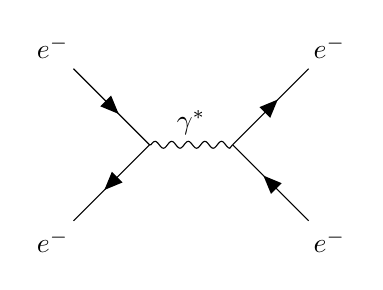
\begin{tikzpicture}
                    \begin{feynman}
                        
                        \vertex (g1);
                        \vertex at ($(g1) + (-3.5em,3.5em) $) (e1) {\(e^-\)};
                        \vertex at ($(g1) + (-3.5em,-3.5em) $) (e2) {\(e^-\)};
    
                        \vertex at ($(g1) + (3em,0)$) (g2) ;
                        \vertex at ($(g2) + (3.5em,3.5em) $) (m1) {\(e^-\)};
                        \vertex at ($(g2) + (3.5em,-3.5em) $) (m2) {\(e^-\)};
                        \diagram* {
                            {[edges=fermion]
                              (e1) -- (g1) -- (e2),
                              (m2) -- (g2) -- (m1)
                            },
                            (g1) -- [boson, edge label =\(\gamma^\ast\)] (g2)
                        };
    
                    \end{feynman}
                \end{tikzpicture}
            }
        \end{center} \columnbreak
        \item the negative energy solutions of the Dirac equation are interpreted as positive energy antiparticles propa- gating forwards in time
        \begin{center}
            \scalebox{1.25}{
                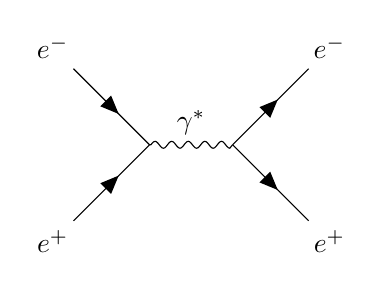
\begin{tikzpicture}
                    \begin{feynman}
                        
                        \vertex (g1);
                        \vertex at ($(g1) + (-3.5em,3.5em) $) (e1) {\(e^-\)};
                        \vertex at ($(g1) + (-3.5em,-3.5em) $) (e2) {\(e^+\)};
    
                        \vertex at ($(g1) + (3em,0)$) (g2) ;
                        \vertex at ($(g2) + (3.5em,3.5em) $) (m1) {\(e^-\)};
                        \vertex at ($(g2) + (3.5em,-3.5em) $) (m2) {\(e^+\)};
                        \diagram* {
                            {[edges=fermion]
                              (e1) -- (g1),  (e2) -- (g1),
                              (g2) -- (m2) , (g2) -- (m1)
                            },
                            (g1) -- [boson, edge label =\(\gamma^\ast\)] (g2)
                        };
    
                    \end{feynman}
                \end{tikzpicture}
            }
        \end{center}
    \end{enumerate}
\end{multicols}
\end{solution}

\noindent\rule{7in}{1.5pt}

%%%%%%%%%%%%%%%%%%%%%%%%%%%%%%%%%%%%%%%%%%%%%%%%%%%%%%%%%%%%%%%%%%%%%%%%%%%%%%%%%%%%%%%%%%%%%%%%%%%%%%%%%%%%%%%%%%%%%%%%%%%%%%%%%%%%%%%%

\begin{problem}{4.12}
Verify that the helicity operator
\begin{align*}
    \hat{h} = \frac{\hat{\boldsymbol{\Sigma}}\cdot\hat{\boldp}}{2p} = \frac{1}{2p}
    \begin{pmatrix}
        \boldmath{\sigma}\cdot\hat{\boldp} & 0 \\
        0 & \boldmath{\sigma}\cdot\hat{\boldp}
    \end{pmatrix}
\end{align*}
commutes with the Dirac Hamiltonian,
\begin{align*}
    \hat{H}_D = \boldsymbol{\alpha}\cdot\hat{\boldp} + \beta m
\end{align*}
\end{problem}
\begin{solution}
The commutation between $\hat{h}$ and $\hat{H}_D$ could be written as,

\begin{align*}
    [ \hat{H}_D , \hat{h} ] &= \frac{1}{2p} \left[\boldsymbol{\alpha}\cdot\hat{\boldp} + \beta m,  \hat{\boldsymbol{\Sigma}}\cdot\hat{\boldp} \right] \\[0.15in]
                            &= \frac{1}{2p}   \left[ \boldsymbol{\alpha}\cdot\hat{\boldp} , \hat{\boldsymbol{\Sigma}}\cdot\hat{\boldp}   \right] + \frac{m}{2p} \left[\beta,\hat{\boldsymbol{\Sigma}}\cdot\hat{\boldp} \right] 
\end{align*}\\
Let us first evaluate the second commutator : 

\begin{align*}
    \left[\beta,\hat{\boldsymbol{\Sigma}}\cdot\hat{\boldp} \right] &= \left[\beta,\Sigma_i \hatp_i\right] \\
    &= \cancelto{0}{\left[\beta,\Sigma_i\right]\hatp_i} + \Sigma_i \cancelto{0}{\left[ \beta,\hatp_i \right]}
\end{align*}\\
where the second term is eliminated due to the fact that matrix operation and differentiation could be commuted (one could check oneself by operating on an arbitrary spinor). The first commutator then could be again reduced into,

\begin{align*}
    \left[ \boldsymbol{\alpha}\cdot\hat{\boldp} , \hat{\boldsymbol{\Sigma}}\cdot\hat{\boldp}   \right] &= \left[ \alpha_i\hat{p}_i , \Sigma_j \hat{p}_j \right] \\[0.1in]
    &= \alpha_i \cancelto{0}{\left[ \hatp_i,\Sigma_j \right]}\hatp_j + \alpha_i \Sigma_j \cancelto{0}{\left[ \hatp_i,\hatp_j \right]} + \left[\alpha_i,\Sigma_j\right]\hatp_j\hatp_i + \Sigma_j \cancelto{0}{\left[ \alpha_i,\hatp_j \right]} \hatp_i \\[0.1in]
    &=  2i \epsilon_{ijk}\alpha_k \hatp_j \hatp_i    = 2i\epsilon_{ijk}\alpha_k \left(\delta_{ji} - \hatp_i\hatp_j\right) = 2i \epsilon_{ijk}\alpha_k \hatp_i \hatp_j \\[0.1in]
    &= 0 \qed 
\end{align*}
\end{solution}

\noindent\rule{7in}{1.5pt}

%%%%%%%%%%%%%%%%%%%%%%%%%%%%%%%%%%%%%%%%%%%%%%%%%%%%%%%%%%%%%%%%%%%%%%%%%%%%%%%%%%%%%%%%%%%%%%%%%%%%%%%%%%%%%%%%%%%%%%%%%%%%%%%%%%%%%%%%

\begin{problem}{4.13}
Show that
\begin{align*}
     \mathsf{P} u_\uparrow \left( \theta,\phi \right) = u_\downarrow \left( \pi-\theta,\pi+\phi \right)
\end{align*}
and comment on the result.
\end{problem}
\begin{solution}
One could straightforwardly write down,

\begin{align*}
    \mathsf{P}u_\uparrow\left(\theta,\phi\right) = \gamma^0 u_\uparrow\left(\theta,\phi\right) &= N \gamma^0 \begin{pmatrix}[1.5] 
        \cos \frac{\theta}{2} \\
        e^{i\phi} \sin \frac{\theta}{2} \\
        \frac{p}{E+m} \cos \frac{\theta}{2} \\
        \frac{p}{E+m} e^{i\phi} \sin \frac{\theta}{2} \\
    \end{pmatrix} = N  \begin{pmatrix}[1.5] 
        \cos \frac{\theta}{2} \\
        e^{i\phi} \sin \frac{\theta}{2} \\
        -\frac{p}{E+m} \cos \frac{\theta}{2} \\
        -\frac{p}{E+m} e^{i\phi} \sin \frac{\theta}{2} \\
    \end{pmatrix} \\[0.15in]
    &= N  \begin{pmatrix}[1.5] 
        - \sin \left(\frac{\pi}{2} - \frac{\theta}{2}\right) \\
        e^{i(\pi+\phi)} \cos \left(\frac{\pi}{2} - \frac{\theta}{2}\right) \\
         \frac{p}{E+m} \sin \left(\frac{\pi}{2} - \frac{\theta}{2}\right) \\
        -\frac{p}{E+m} e^{i(\pi+\phi)} \cos  \left(\frac{\pi}{2} - \frac{\theta}{2}\right) \\
    \end{pmatrix} \\[0.15in]
    &= u_\downarrow \left( \pi-\theta,\pi+\phi\right) \qed
\end{align*}\\
One could notice that in terms of spherical angles, the result above shows that the parity operator actually flips the momentum direction to $-\boldp$, which will result in the opposite helicity.
\end{solution}

\noindent\rule{7in}{1.5pt}

%%%%%%%%%%%%%%%%%%%%%%%%%%%%%%%%%%%%%%%%%%%%%%%%%%%%%%%%%%%%%%%%%%%%%%%%%%%%%%%%%%%%%%%%%%%%%%%%%%%%%%%%%%%%%%%%%%%%%%%%%%%%%%%%%%%%%%%%

\begin{problem}{4.14}
Under the combined operation of parity and charge conjugation $(\mathsf{CP})$ spinors transform as
\begin{align*}
    \psi \to \psi^C = \mathsf{CP} \psi = i \gamma^2\gamma^0 \psi^\ast 
\end{align*}
Show that up to an overall complex phase factor
\begin{align*}
    \mathsf{CP} u_\uparrow \left( \theta,\phi \right) = v_\downarrow  \left( \pi-\theta,\pi+\phi \right)
\end{align*}
\end{problem}
\begin{solution}

\end{solution}

\noindent\rule{7in}{1.5pt}

%%%%%%%%%%%%%%%%%%%%%%%%%%%%%%%%%%%%%%%%%%%%%%%%%%%%%%%%%%%%%%%%%%%%%%%%%%%%%%%%%%%%%%%%%%%%%%%%%%%%%%%%%%%%%%%%%%%%%%%%%%%%%%%%%%%%%%%%

\begin{problem}{4.15}
Starting from the Dirac equation, derive the identity
\begin{align*}
    \overbar{u}  (p') \gamma^\mu u ( p ) = \frac{1}{2m} \overbar{u}(p') \left(p+p'\right) u(p) + \frac{i}{m} \overbar{u}\left(p'\right) \Sigma^{\mu\nu} q_\nu u(p)
\end{align*}
where $q = p'-p$ and $\Sigma^{\mu\nu}=\frac{i}{4}\left[ \gamma^\mu,\gamma^\nu \right]$
\end{problem}
\begin{solution}
Using the Dirac equation for $u(p)$, one could write down $\overbar{u}(p')\gamma^\mu u(p)$ as,

\begin{align}
    \overbar{u}(p')\gamma^\mu u(p) &= \frac{1}{m}  \overbar{u}(p')\gamma^\mu \slashed{p} u(p)  \label{4.15.1} \\[0.15in]
                                   &= \frac{1}{m}  \overbar{u}(p')\gamma^\mu \gamma^\nu p_\nu u(p) \nonumber \\[0.15in]
                                   &= \frac{1}{m}  \overbar{u}(p')\left( 2g^{\mu\nu} - \gamma^\nu \gamma^\mu \right) p_\nu u(p) \nonumber \\[0.15in]
                                   &= \frac{2}{m}  \overbar{u}(p') p^\mu  u(p) - \frac{1}{m}  \overbar{u}(p') \slashed{p} \gamma^\mu   u(p)    \label{4.15.2}
\end{align}\\
One could do the same using the Dirac equation for the adjoint case,

\begin{align}
    \overbar{u}(p')\gamma^\mu u(p) &= \frac{1}{m}  \overbar{u}(p')  \slashed{p'} \gamma^\mu u(p)  \label{4.15.3} \\[0.15in]
                                   &= \frac{1}{m}  \overbar{u}(p')\gamma^\nu \gamma^\mu p'_\nu u(p) \nonumber \\[0.15in]
                                   &= \frac{1}{m}  \overbar{u}(p')\left( 2g^{\nu\mu} - \gamma^\mu \gamma^\nu \right) p'_\nu u(p) \nonumber \\[0.15in]
                                   &= \frac{2}{m}  \overbar{u}(p') p'^\mu  u(p) - \frac{1}{m}  \overbar{u}(p') \gamma^\mu   \slashed{p'} u(p)   \label{4.15.4}
\end{align}\\
Using the above relations one could again express  $\overbar{u}(p')\gamma^\mu u(p)$ as,

\begin{align}
    \overbar{u}(p')\gamma^\mu u(p) &= \frac{1}{2} \left\{ \frac{1}{m}  \overbar{u}(p')\gamma^\mu \slashed{p} u(p)  + \frac{1}{m}  \overbar{u}(p')  \slashed{p'} \gamma^\mu u(p) \right\} \nonumber \\[0.15in]
                                   &= \frac{1}{m}   \overbar{u}(p') (p+p')^\mu  u(p)  - \frac{1}{2m} \overbar{u}(p') \left\{ \slashed{p}\gamma^\mu + \gamma^\mu \slashed{p'} \right\}  u(p) \label{4.15.5}
\end{align}\\
Before moving on, one could again use another relation that could be derived from (\ref{4.15.1}) to (\ref{4.15.4}) as :

\begin{align}
    (\ref{4.15.1}) = (\ref{4.15.2}) &\implies \frac{1}{m}  \overbar{u}(p')\gamma^\mu \slashed{p} u(p) = \frac{2}{m}  \overbar{u}(p') p^\mu  u(p) - \frac{1}{m}  \overbar{u}(p') \slashed{p} \gamma^\mu   u(p) \nonumber \\[0.15in]
                                    &\implies 2 \overbar{u}(p') p^\mu  u(p) = \overbar{u}(p') \left\{ \gamma^\mu \slashed{p} + \slashed{p}\gamma^\mu \right\} u(p)  \label{4.15.6} \\[0.15in]
    (\ref{4.15.3}) = (\ref{4.15.4}) &\implies  \overbar{u}(p')  \slashed{p'} \gamma^\mu u(p)  = \frac{2}{m}  \overbar{u}(p') p'^\mu  u(p) - \frac{1}{m}  \overbar{u}(p') \gamma^\mu   \slashed{p'} u(p)    \nonumber \\[0.15in]
                                    &\implies 2 \overbar{u}(p') p'^\mu  u(p) = \overbar{u}(p') \left\{ \gamma^\mu \slashed{p'} + \slashed{p'}\gamma^\mu \right\} u(p)   \label{4.15.7}
\end{align}\\
Adding up both (\ref{4.15.6}) and (\ref{4.15.7}) gives, 

\begin{align}
    \overbar{u}(p') (p+p')^\mu  u(p) = \frac{1}{2} \overbar{u}(p') \left\{ \gamma^\mu \slashed{p'} + \slashed{p'}\gamma^\mu + \gamma^\mu \slashed{p} + \slashed{p}\gamma^\mu \right\} u(p) \label{4.15.8}
\end{align}\\
Plugging (\ref{4.15.8}) into (\ref{4.15.5}) but splitting the first term into half gives, 

\begin{align}
    \overbar{u}(p')\gamma^\mu u(p) &=   \frac{1}{2m}   \overbar{u}(p') (p+p')^\mu  u(p) + \frac{1}{2m}   \overbar{u}(p') (p+p')^\mu  u(p)  - \frac{1}{2m} \overbar{u}(p') \left\{ \slashed{p}\gamma^\mu + \gamma^\mu \slashed{p'} \right\}  u(p)  \nonumber \\[0.15in]
                                   &=   \frac{1}{2m}   \overbar{u}(p') (p+p')^\mu  u(p) + \frac{1}{4m} \overbar{u}(p') \left\{ \gamma^\mu \slashed{p'} + \slashed{p'}\gamma^\mu + \gamma^\mu \slashed{p} + \slashed{p}\gamma^\mu \right\} u(p) - \frac{1}{2m} \overbar{u}(p') \left\{ \slashed{p}\gamma^\mu + \gamma^\mu \slashed{p'} \right\}  u(p)  \nonumber \\[0.15in]
                                   &=   \frac{1}{2m}   \overbar{u}(p') (p+p')^\mu  u(p) - \frac{1}{4m} \overbar{u}(p') \left\{  \gamma^\mu \slashed{p'} - \slashed{p'}\gamma^\mu - \gamma^\mu \slashed{p} + \slashed{p}\gamma^\mu \right\} u(p)  \nonumber \\[0.15in]
                                   &=   \frac{1}{2m}   \overbar{u}(p') (p+p')^\mu  u(p) - \frac{1}{4m} \overbar{u}(p') \left\{ \gamma^\mu (\slashed{p'}-\slashed{p}) - (\slashed{p'}-\slashed{p}) \gamma^\mu \right\} u(p)  \nonumber \\[0.15in]
                                   &=   \frac{1}{2m}   \overbar{u}(p') (p+p')^\mu  u(p) - \frac{1}{4m} \overbar{u}(p') \left[  \gamma^\mu , \slashed{q} \right] u(p)  \nonumber \\[0.15in]
                                   &=   \frac{1}{2m}   \overbar{u}(p') (p+p')^\mu  u(p) - \frac{1}{4m} \overbar{u}(p') \left[  \gamma^\mu , \gamma^\nu \right] q_\nu u(p)  \nonumber \\[0.15in]
                                   &=   \frac{1}{2m}   \overbar{u}(p') (p+p')^\mu  u(p) + \frac{i}{m} \overbar{u}\left(p'\right) \Sigma^{\mu\nu} q_\nu u(p) \qed \nonumber
\end{align}
\end{solution}

\noindent\rule{7in}{1.5pt}

%%%%%%%%%%%%%%%%%%%%%%%%%%%%%%%%%%%%%%%%%%%%%%%%%%%%%%%%%%%%%%%%%%%%%%%%%%%%%%%%%%%%%%%%%%%%%%%%%%%%%%%%%%%%%%%%%%%%%%%%%%%%%%%%%%%%%%%%


\end{document}
 